\documentclass[a4paper]{article}%{{{

\usepackage[utf8]{inputenc}
\usepackage[T1]{fontenc}
\usepackage{textcomp}
\usepackage{url}
\usepackage{hyperref}
\usepackage[top=2.5cm,bottom=2.5cm,right=2cm,left=3cm]{geometry}
\usepackage[french]{babel}
\usepackage[backend=biber,style=ieee]{biblatex}
\usepackage{glossaries}
%\usepackage{titletoc}% http://ctan.org/pkg/titletoc
\usepackage{qtree}
\usepackage{listings}
\usepackage{xcolor}
\usepackage{setspace}
\usepackage{graphicx}
\usepackage{geometry}
\usepackage{titlesec}
\usepackage{chngcntr}
\counterwithin*{section}{part}

\addbibresource{refs.bib}

\definecolor{codegreen}{rgb}{0,0.6,0}
\definecolor{codegray}{rgb}{0.5,0.5,0.5}
\definecolor{backcolour}{rgb}{0.95,0.95,0.92}
\definecolor{backpink}{rgb}{1,0.94,0.95}

\lstdefinestyle{codestyle}{
    backgroundcolor=\color{backcolour},
    commentstyle=\color{codegreen},
    keywordstyle=\color{magenta},
    numberstyle=\tiny\color{codegray},
    stringstyle=\color{teal},
    basicstyle=\ttfamily\footnotesize,
    breakatwhitespace=false,
    breaklines=true,
    captionpos=b,
    keepspaces=true,
    %numbers=left,
    %numbersep=5pt,
    showspaces=false,
    showstringspaces=false,
    showtabs=false,
    tabsize=2
}

\lstdefinestyle{grammarstyle}{
    backgroundcolor=\color{backpink},
    commentstyle=\color{codegreen},
    keywordstyle=\color{purple},
    numberstyle=\tiny\color{codegray},
    stringstyle=\color{teal},
    basicstyle=\ttfamily\footnotesize,
    breakatwhitespace=false,
    breaklines=true,
    captionpos=b,
    keepspaces=true,
    %numbers=left,
    %numbersep=5pt,
    showspaces=false,
    showstringspaces=false,
    showtabs=false,
    tabsize=2
}

\lstnewenvironment{code}[1][]
  {\noindent\minipage{\linewidth}\medskip
   \lstset{basicstyle=\ttfamily\footnotesize,frame=single,#1,upquote=true}
    \lstset{style=codestyle}
     }
  {\endminipage}

 \lstnewenvironment{grammar}[1][]
  {\noindent\minipage{\linewidth}\medskip
   \lstset{basicstyle=\ttfamily\footnotesize,frame=single,#1,upquote=true}
   \lstset{style=grammarstyle}
   }
  {\endminipage}

%===========style & geometry===========
%\lstset{style=mystyle}

 \geometry{
 a4paper,
  left=30mm,
  right=20mm,
  top=25mm,
  bottom=25mm,
 }

 \titleformat*{\section}{\LARGE\bfseries}
 \titleformat*{\subsection}{\Large\bfseries}

%================infos=================
\pagenumbering{gobble}
\begin{titlepage}

\title{Création d'un langage interprété}
\author{Franck ALONSO, CHASSAGNOL Rémi}
\date{\today}
\end{titlepage}
%}}}
%===============Glossaire==============
\makeglossaries
\newglossaryentry{ast}
{
    name=AST,
    description={(Abstract Syntax Tree) structure sous forme d'arbre utilisée
                 pour représenter une grammaire.}
}
\newglossaryentry{bnf}
{
    name=forme de Backus-Naur,
    description={métalangage utilisé pour décrire les langages de programmation.}
}
\newglossaryentry{varFonc}
{
    name=fonctions variadiques,
    description={fonction qui prend un nombre indéfini de paramètres.}
}
\newglossaryentry{bytecode}
{
    name=bytecode,
    description={code intermédiaire entre les instructions machine et le code
    source. Il n'est pas directement exécutable par l'ordinateur.}
}
\newglossaryentry{gc}
{
    name=garbage collector,
    description={(ramasse-miettes) outil inventé par John McCarthy qui permet
    de collecter les zones mémoires non utilisées lors de l'exécution d'un
    programme.}
}
\newglossaryentry{lexer}
{
    name=lexeur,
    description={ Le lexeur, ou encore appelé analyseur lexical, a pour but de
    transformer le texte du code source en des unités lexicales, appelées
    \textit{tokens}.}
}
\newglossaryentry{parser}
{
    name=parseur,
    description={Également appelé analyseur syntaxique, son rôle principal est la vérification de
    la syntaxe du code en regroupant les tokens selon une structure suivant des
    règles syntaxiques.}
}
\newglossaryentry{shebang}
{
    name=Shebang,
    description={représenté par \textbf{\#!}, il se place en haut du fichier et
    permet sur les systèmes UNIX de déclarer que le fichier est un script et
    indique quel interpréteur doit être utilisé lors d'une exécution.}
}



%------------------------------------------------------------------------------%
%                                  Title page                                  %
%------------------------------------------------------------------------------%
\pagestyle{empty}
\begin{document}
\begin{titlepage}
    
\includegraphics{img/logo_isima_inp.jpeg}
       \begin{center}
           \vspace*{1cm}
               
           \Huge
           \textbf{Création d'un langage interprété}
               
           \vspace{0.5cm}
           \LARGE
           Rapport d'élève ingénieur\\
           Projet de 2\up{ème} année\\
           Filière F2 : Génie Logiciel et Systèmes Informatiques
               
           \vspace{1.5cm}
               
           Présenté par : \textbf{Franck ALONSO} et \textbf{Rémi CHASSAGNOL}
               
           \vfill
               
           \vspace{0.5cm}
         \end{center}          
   
               
           \large
           \noindent
           Responsable ISIMA : \hfill \textbf{Mardi 31/01/2023}\\~\\
           \raggedleft \textbf{Projet de 60h}\\~\\
           \raggedright
           Campus des Cézeaux. 1 rue de la Chébarde. TSA 60125. 63178 Aubière CEDEX\\
     
               
   
   \end{titlepage}
\clearpage{}

%------------------------------------------------------------------------------%
%                               Table of contents
%------------------------------------------------------------------------------%
\pagenumbering{arabic}
\thispagestyle{empty}
\tableofcontents
\clearpage{}

%------------------------------------------------------------------------------%
%                                Remerciements
%------------------------------------------------------------------------------%
\section*{Remerciements}
\thispagestyle{empty}
\addcontentsline{toc}{section}{Remerciements}

\doublespacing
\large

Nous tenons à remercier Loïc YON pour nous avoir guidé et conseillé lors de la
réalisation du projet. Nous remercions aussi Murielle MOUZAT pour l'aide qu'elle
nous a fourni à travers son cours pour la rédaction de ce rapport. Parmi nos
professeurs, nous souhaitons aussi remercier Alexis PEREDA pour ses conseils sur
l'utilisation de C++ et pour avoir partagé ses connaissances sur les
compilateurs ainsi que Yves-Jean DANIEL pour nous avoir conseillé l'utilisation
de Flex et Bison pour l'écriture d'un \gls{parser}.

\normalsize
\onehalfspacing

\clearpage{}

%------------------------------------------------------------------------------%
%                               Table of figures
%------------------------------------------------------------------------------%
\listoffigures
\clearpage{}


%------------------------------------------------------------------------------%
%                              Résumé et Abstract
%------------------------------------------------------------------------------%
%\setcounter{secnumdepth}{3}
\section*{Résumé}
\addcontentsline{toc}{section}{Résumé}

Ce projet s'inscrit dans le cadre du projet commun de la filière génie logiciel
dont l'objectif est la création d'outils de démonstration servant à présenter la
filière. Notre travail a consisté en la création d'un langage de programmation
transpilé simple avec une syntaxe similaire à celle du C. Le programme doit lire
un fichier de code source et le traduire en code python. Il doit être capable
de détecter les erreurs de syntaxe et de les spécifier à l'utilisateur. De
plus, le langage est à typage statique, de ce fait, le programme doit aussi être
capable de détecter les erreurs de types.\\

Le développement a été réalisé avec le langage C++ et emploie le paradigme objet.
De plus, nous avons utilisé les outils GNU Flex et GNU Bison pour la création du
parseur. À noter que le programme ne nécessite pas de système d'exploitation
particulier, cependant, il requiert l'installation des outils cités précédemment
ainsi qu'une version de python3 pour fonctionner.\\

Au final nous avons réussi à implémenter un parseur fonctionnel ainsi que tous
les éléments du langage excepté l'inclusion de bibliothèques. Pour le
transpileur, nous avons pu fournir une solution très simpliste qui ne correspond
cependant pas à ce que l'on pourrait trouver sur un vrai transpileur. Le projet
n'est donc pas entièrement terminé mais il présente tout de même une partie de
solution et permet bien de traduire notre code en python.
\\~\\

\noindent
Mots-clés : \textbf{C++}, \textbf{transpileur}, \textbf{lexeur}, \textbf{parseur},
\textbf{flex}, \textbf{bison},  \textbf{langage de programmation}

\section*{Abstract}
\addcontentsline{toc}{section}{Abstract}

This project is a part of the common project of the software development
pathway. The objective is to create a tool for presenting software development.
Our work consisted in the creation of a simple transpiled programming language
with a syntax similar to C language. The program has to be able to read a source
code file and generate a python program. It must detect syntax errors in the and
report theme to the user. Furthermore, the language is statically typed so the
program also has to detect and report type errors.\\

The development has been done using C++ and object oriented programming.
Moreover, we have used the tools GNU Flex and GNU Bison to generate our parser.
We can notice that the program doesn't require any particular operating system,
however the tools previously quoted and a version of python3 have to be
installed.\\

In the end we've been able to implement a parser and all the elements of our
language without libraries inclusions. For the transpiler, we've made a very
simple solution that doesn't correspond to what we could expect of a real
transpiler. The project is not completely finished, however, it presents a piece
of solution and the program eventualy is able to translate our code in python.
\\~\\

\noindent
Keywords : \textbf{C++}, \textbf{transpiler}, \textbf{lexer}, \textbf{parser},
\textbf{flex}, \textbf{bison}, \textbf{programming language}

\clearpage{}

%------------------------------------------------------------------------------%
%                                 Introduction
%------------------------------------------------------------------------------%
\pagestyle{plain}
\setcounter{page}{1}
\clearpage
\section*{Introduction}
\addcontentsline{toc}{section}{Introduction}
\large
Dans le cadre du projet de 2\up{ème} année à l'ISIMA, nous avons choisi de
réaliser un travail concernant le sujet commun de la filière 2, génie logiciel
et systèmes d'informations. Le but du projet commun est la création d'outils de
démonstration servant à présenter la filière.\\

Nous souhaitions au départ, créer un langage de programmation interprété ainsi
qu'un IDE, cependant, ce projet s'est avéré trop ambitieux pour être réalisé en
60 heures. Pour simplifier, nous avons décidé de concevoir un langage transpilé,
délégant ainsi une partie des tâches complexes comme la gestion de la mémoire à
un compilateur existant.\\

Ce projet permettra de présenter un langage de programmation très simple pour
introduire des lycéens à la programmation. De plus, il pourra constituer une
maquette pour les élèves de l'ISIMA souhaitant étudier le fonctionnement des
compilateurs.\\

Pour présenter ce projet, nous commencerons par la forme du langage à créer
souhaitée, puis nous détaillerons sa structure. Une fois familiarisés avec les
différentes étapes de son implémentation,  nous introduirons les concepts et
outils qui permettent la réalisation de notre langage.\\

\normalsize
\clearpage{}

%------------------------------------------------------------------------------%
%                                     Plan                                     %
%------------------------------------------------------------------------------%

% NOTE: les partie ne sont pas très équilibrées

\part{Contexte du projet}

\section{Concept de langage transpilé}

L'objectif du projet commun est de créer un outil qui pourra servir à faire des
démonstrations pour présenter la filière génie logiciel. Étant donné le fait que
le code fait partie intégrante du développement logiciel nous avons décidé de
créer un langage de programmation simple pouvant servir à l'initiation au
développement ainsi qu'à certains concepts relatifs aux langages de
programmation.\\

Il existe quatre familles de langages de programmation. La première est celle
des langages compilés comme le C ou le C++. Le principe est de transformer le
code source en assembleur puis de générer un exécutable. Cette méthode est la
plus complexe, cependant les langages compilés sont généralement les plus
rapides et les plus légers.

La seconde méthode pour exécuter du code est l'utilisation d'une machine
virtuelle. Le code source du langage est traduit en un code de bas niveau, le
\gls{bytecode}, qui est ensuite exécuté par une machine virtuelle. C'est par
exemple le cas du langage Java.

La troisième famille est celle des langages interprétés. Ici c'est
l'interpréteur qui se charge directement de l'exécution du code source, sans
passer par une représentation intermédiaire comme le bytecode.

La dernière famille est celle que nous allons étudier lors de la réalisation de
ce projet, ce sont les langages transpilés. L'objectif d'un transpileur est de
traduire le code source dans un autre langage. Le principal avantage du
transpileur est qu'il permet de déléguer les tâches complexes au compilateur du
langage cible. Par exemple, cela évite d'avoir à écrire un \gls{gc} pour gérer
la mémoire.

\section{Les fonctionnalités du langage}

Notre objectif global est de pouvoir écrire du code dans un fichier puis
utiliser notre transpileur pour générer un fichier python (qui sera exécuté avec
python3). Le langage doit être simple mais doit tout de même posséder les
fonctionnalités suivantes :

Le langage doit permettre le stockage d'informations dans des variables. Nous
souhaitons que notre langage possède trois types de données, les caractères, les
entiers et les flottants. Étant donné que l'objectif du projet est de pouvoir
présenter la programmation, il est intéressant d'utiliser un langage qui possède
des types car cela permet de mieux comprendre comment l'ordinateur gère les
données.

On doit aussi avoir la possibilité d'écrire des fonctions et des procédures
paramétrées qui pourront être utilisées dans différents endroits du programmes.
Ces procédures et fonctions pourront contenir une suite d'instructions dans un
bloc de code.

De plus, le langage devra posséder des structures de contrôle permettant la
création de conditions et de boucles.

Enfin, il doit intégrer des fonctions arithmétiques permettant les
opérations de base, des fonctions booléennes permettant de faire des
tests ainsi que des fonctions permettant des actions d'entrée et de sortie
(affichage et récupération de données via la console).

Étant donné le fait que notre langage pourra être utilisé pour faire des
présentations lors de portes ouvertes, nous souhaitons aussi que la syntaxe soit
assez éloignée de celle du langage python. Le but étant de pouvoir présenter
un langage différent à des lycéens qui ont pour la plupart déjà utilisé python.

\section{Analyse du problème}

Nous souhaitons créer un langage simple qui peut être écrit dans un fichier, la
première chose à faire va donc être de définir sa syntaxe. La syntaxe du langage
va dépendre des fonctionnalités décrites plus haut. Il faudra donc un moyen de
déclarer des variables, des fonctions ou encore un moyen de délimiter les
instructions.

Étant donné le fait que notre langage doit être écrit dans un fichier texte, il
faudra un moyen d'extraire les informations contenues dans le texte. L'outil
généralement utilisé pour ce type de tâche s'appelle un parseur, qui va
permettre de reconnaître des règles de grammaire dans le code source. Nous avons
décidé de ne pas implémenter de parseur par nous même mais plutôt d'utiliser
deux outils qui vont permettre la génération du code du parseur : Flex et Bison.
Ces deux outils vont nous permettre de gagner du temps et d'avoir un code
beaucoup plus efficace car les codes qu'ils génèrent sont très performants.

Ensuite, il nous faudra un moyen de représenter les différentes instructions
récupérées par le parseur. Pour ce faire, il existe plusieurs méthodes
comme par exemple, récupérer des instructions bas niveau (proche de
l'assembleur) pour construire un programme. Une autre solution serait d'utiliser
la programmation orientée objet pour gérer toutes les instructions du programme.
Nous choisirons l'approche objet car il sera beaucoup plus simple de générer le
code python au moment de la transpilation. Le code bas niveau aurait peut-être
été un meilleur choix si nous avions implémenté un interpréteur ou un
compilateur.

Le code python généré par le transpileur ne doit pas contenir d'erreurs de
syntaxe ou de problème de définitions de variables ou de fonctions. Il faudra
donc faire toutes les vérifications nécessaires au préalable. Pour ce faire,
nous devrons trouver les erreurs de syntaxe dans le programme de base ainsi que
faire des vérifications sur la définition et le type des différents éléments. La
traduction du code ne devra se faire que si le programme de base ne comporte
aucune erreur. Il faudra donc un moyen de récupérer les erreurs de compilations
ainsi qu'une table des symboles pour vérifier les définitions et les types.

Pour la traduction du code il y a aussi plusieurs possibilités. Avec le modèle
objet, on peut avoir un transpileur qui se charge de traduire les différents
éléments ou avoir des méthodes de traduction pour chacun des éléments du
programme. Il sera peut-être aussi nécessaire de modifier le programme récupéré
avant la traduction. À noter que l'objectif du projet est de créer un langage
assez simple, il n'y aura donc pas d'optimisation avant la traduction. Par
manque de temps, nous choisirons l'option d'avoir des méthodes de traduction des
objets représentant éléments du langage.\\

Pour mener à bien le projet, il nous faudra donc un parseur pour reconnaître la
grammaire du langage et un moyen de représenter et de stocker les éléments du
langage. Il nous faudra aussi un moyen de collecter les erreurs et une table des
symboles pour vérifier les définitions et les types. Enfin il faudra faire la
traduction des éléments du langage en code python.

\clearpage
\part{Réalisation et conception}

\section{Conception des éléments du langage}

\subsection{Définition de la grammaire}

Avant d'implémenter notre langage, il faut avoir une idée de sa grammaire.
Puisque nous souhaitons utiliser ce langage à des fins pédagogiques, nous avons
décidé de simplifier au maximum la syntaxe. Par exemple, nous avons choisi de
supprimer tous les opérateurs, ainsi, toutes les opérations arithmétiques et
booléennes auront la même syntaxe que les fonctions. Par exemple, $a+b$ s'écrira
\textit{add}(a, b). De plus, pour différer au maximum de python, notre syntaxe
s'inspirera de celle des langages C et Rust. Pour définir la grammaire de
manière formelle, nous utiliserons la \gls{bnf}.

\subsubsection*{Les variables}

Pour stocker des données, notre langage utilise des variables dont la
convention de nommage est la même qu'en \textbf{C}. Le langage est à typage
statique, ce qui signifie que toutes les variables doivent être déclarées avec
un type avant d'être utilisées. Pour l'instant, nous possédons trois types :
les entiers (\textit{int}), les nombres à virgule flottante (\textit{flt}) et les
caractères (\textit{chr}). Voici la syntaxe pour déclarer une variable:

\begin{grammar}
<identifier> ::= 'a'-'z'( <alpha> | '0'-'9' )*
<int> ::= "int"
<flt> ::= "flt"
<chr> ::= "chr"
<type> ::= <int> | <flt> | <chr>
<declaration> ::= <type> <identifier> ";"
\end{grammar}\leavevmode\newline

A noter qu'ici, on a une légère différence avec le C pour le nom des fonctions
et des variables (\textbf{identifier} ici). En effet, le C permet aux noms de
variables et de fonctions de pouvoir commencer par une majuscule. Ici, nous
avons décidé de forcer les noms à commencer par une lettre minuscule, le non
respect de cette règle entrainera une erreur de syntaxe. Le but étant d'une part
de différer encore plus de python et d'autre part de forcer l'application de
notre guide de style.

\subsubsection*{Les fonctions}

La syntaxe pour les fonctions est la même qu'en Rust. Pour définir des
fonctions, nous utilisons le mot clé \textbf{fn}, suivit du nom de la fonction
avec ses paramètres entre parenthèses et enfin le bloc de code qui contient
les instructions entre accolades. De plus, il faut spécifier le type de la valeur
de retour de la fonction en utilisant \textbf{-> type} quand c'est nécessaire.

\begin{grammar}
<function> ::= fn <identifier>"("<parameters>")" [ "->" <type> ] "{"<instructions>"}"
\end{grammar}\leavevmode\newline

Pour pouvoir retourner une valeur, il faudra utiliser le mot clé \textit{return}
dans la fonction.

\subsubsection*{Les structures de contrôle}

Nous avons aussi ajouté les structures de contrôle présentes dans la plupart des
langages de programmation. Il y a une structure \textit{if} qui permet de tester
une condition. Un \textit{if} peut-être suivit d'un bloc \textit{else} si
besoin. À noter cependant que cette grammaire n'autorise pas les \textit{else
if}, dans ce cas il faudra mettre la nouvelle condition à l'intérieur du bloc
de code du \textit{else}. La grammaire autorise aussi les boucles
\textit{while}, et la syntaxe est la même qu'en C. Enfin, il y a la boucle
\textit{for} qui utilise la règle \textit{range} qui contient trois valeurs
séparées par des virgules. Ces trois valeurs correspondent au début et à la fin
de boucle et au pas. Par exemple, \lstinline{range(0, 10, 1)} va générer une
boucle où la variable de boucle prendra les valeurs de 0 à 9 avec un pas de 1.
Il est obligatoire de toujours spécifier ces trois valeurs au \textit{range}.

\begin{grammar}
<if> ::= if "("<condition>")" "{"<instructions>"}" [ else "{" <instructions>"}" ]

<while> ::= while "("<condition>")" "{" <instructions> "}"

<range> ::= range "("<valueSymbol>, <valueSymbol>, <valueSymbol>")"
<for> ::= for <identifier> in <range> "{"<instructions>"}"
\end{grammar}\leavevmode\newline

On rappel que même si la grammaire ne le précise pas, toute variable doit être
déclarée avant d'être utilisée, il faudra donc déclarer la variable de boucle
utilisée dans un \textit{for}.

\subsubsection*{Les opérations}
\label{sec:operator}

Comme dit précédemment, le langage ne comporte pas d'opérateurs donc toutes
les opérations se font à l'aide de fonctions directement intégrées dans le
transpileur. Voici une liste des opérations possibles :

\begin{center}
\begin{tabular}{ | c | c | }
    \hline
    opération & syntaxe\\
    \hline
    \textbf{a} + \textbf{b} & \textit{add}(\textbf{a}, \textbf{b})\\
    \hline
    \textbf{a} - \textbf{b} & \textit{mns}(\textbf{a}, \textbf{b})\\
    \hline
    \textbf{a} $\times$ \textbf{b} & \textit{tms}(\textbf{a}, \textbf{b})\\
    \hline
    \textbf{a} $\div$ \textbf{b} & \textit{div}(\textbf{a}, \textbf{b})\\
    \hline
    \textbf{a} \textbf{==} \textbf{b} & \textit{eql}(\textbf{a}, \textbf{b})\\
    \hline
    \textbf{a} \textbf{<} \textbf{b} & \textit{inf}(\textbf{a}, \textbf{b})\\
    \hline
    \textbf{a} \textbf{>} \textbf{b} & \textit{sup}(\textbf{a}, \textbf{b})\\
    \hline
    \textbf{a} \textbf{<=} \textbf{b} & \textit{ieq}(\textbf{a}, \textbf{b})\\
    \hline
    \textbf{a} \textbf{>=} \textbf{b} & \textit{seq}(\textbf{a}, \textbf{b})\\
    \hline
    \textbf{not} \textbf{a} & \textit{not}(\textbf{a})\\
    \hline
\end{tabular}
\end{center}

\subsubsection*{Entrée et sortie}

Le langage possède aussi la possibilité d'afficher et de lire du texte depuis la
console. La lecture se fait avec la fonction \textit{read} qui prend en
paramètre une variable qui stockera le résultat. Pour l'affichage, il faudra
utiliser la fonction \textit{print} qui peut être utilisée de deux manières :

\begin{itemize}
  \item \lstinline{print("Hello, World!")} : affiche du texte
  \item \lstinline{print(variable)} : affiche une valeur.
\end{itemize}

Nous n'avons pas implémenté de fonction d'affichage similaire à \textbf{printf}
en C. La première raison est le fait que notre langage ne supporte pas les
\gls{varFonc}. De plus, l'ajout de ce type de fonctions d'affichage nécessite la
gestion d'une chaine de formatage, ce qui aurait grandement augmenté la
complexité de notre grammaire si nous avions voulu l'intégrer directement au
langage. Voici la syntaxe pour ces fonctions :

\begin{grammar}
  <print> ::= print"("<variable>")" | print"("<string>")"
  <read> ::= read"("<variable>")"
\end{grammar}\leavevmode\newline

La règle \textit{string} utilisée ci-dessus correspond à une chaîne de caractères
entourée de guillemets comme montré plus haut.

\subsubsection*{Le programme}

La syntaxe du programme est décrite ci-dessous. Un programme est composé de zéro
ou plusieurs inclusions de fichiers ainsi qu'une ou plusieurs fonctions. La
grammaire n'autorise donc pas l'ajout de code en dehors des fonctions, il ne
sera donc pas possible de faire un programme avec juste une instruction
d'affichage comme en python. De plus, il ne sera pas non plus possible de
déclarer des variables globales.

\begin{grammar}
  <program> ::= <include>* | <function>+
\end{grammar}\leavevmode\newline

\subsubsection*{Exemple de code}

Dans cet exemple, nous disposons de 2 variables \textbf{a} et \textbf{b}. La
variable \textbf{a} est lue par commande de l'utilisateur tandis que la valeur 4
est assignée à \textbf{b}.\\
Nous cherchons ensuite à additionner les 2 variables avec la valeur 5. Nous
avons alors la syntaxe suivante :\\

\begin{itemize}
  \item une fonction \textit{add3} qui additionne les valeurs des 3 paramètres\\
  \item une fonction \textit{affiche} qui affiche sur l'écran le nombre passé en paramètre\\
  \item une fonction \textit{main}, où se trouve toutes les commandes voulues de notre programme\\
\end{itemize}


\begin{grammar}[language=C++]
fn add3(int a, int b, int c) -> int {
    return add(a, add(b, c));
}

fn affiche(int n) {
    print("nombre : ");
    print(n);
}

fn main() {
    int a;
    int b;
    read(a);
    set(b, 4);
    affiche(add3(a, b, 5));
}
\end{grammar}\leavevmode\newline
~\\

Maintenant que nous avons défini la syntaxe du langage nous allons voir
l'implémentation d'un outil qui nous sera utile pour la construction d'un
programme.


\clearpage{}

\subsection{Arbre syntaxique}

Pour donner un sens aux éléments textuels du langage, nous utiliserons une
représentation sous forme d'arbre. On appelle cela un arbre syntaxique ou
\gls{ast}. Les arbres syntaxiques sont nés avec la théorie des langages et comme
on peut le voir dans cet article \cite{compilerTICH}, les AST sont très
utilisés par les compilateurs car ce sont des structures plus simples à
manipuler que du texte. Voici l'arbre syntaxique de la fonction \textit{add3} :

\begin{figure}[h]
  \begin{center}
  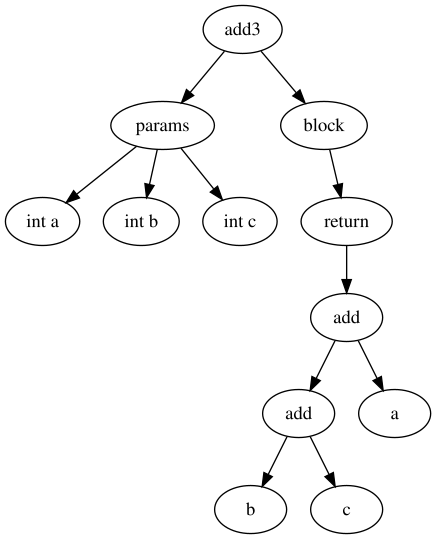
\includegraphics[scale=0.4]{img/ast1.png}
  \caption{Exemple d'arbre syntaxique}
  \end{center}
\end{figure}

Pour cette partie, nous nous sommes inspirés d'un projet appelé \textbf{minijava}
\cite{minijava} ainsi que d'un article \cite{gagnon1998sablecc} qui couvre aussi
l'utilisation des AST en java. Nous avons choisi l'approche objet, avec un AST
représenté par des classes, où chaque nœud de l'arbre a sa propre classe.\\

Toutes les classes de l'arbre sont stockées dans le fichier
\lstinline{AST/AST.hpp} et héritent toutes d'une classe abstraite
\lstinline{ASTNode}. L'emploi de l'héritage ici est important car
nous profiterons par la suite des avantages du polymorphisme pour stocker des
opérations de différents types. La classe \lstinline{ASTNode} est abstraite car
elle ne doit pas être instanciée, il faut que chaque nœud ait un type concret
utilisable dans le transpileur. À noter que l'utilisation du polymorphisme
avec une classe abstraite force l'utilisation de pointeurs et donc d'allocation
dynamique. Étant donné qu'il y a beaucoup d'objets à gérer et que nous n'avons
pas de contrainte particulière en terme de performance mémoire, nous utiliserons
\lstinline{std::shared_ptr} pour gérer tous nos pointeurs. Le diagramme de
classes complet est disponible en annexe \ref{appendix:classAST}. Détaillons
maintenant les parties importantes.

\subsubsection*{Les blocs de code}

La classe \lstinline{Block} correspond aux blocs de code entre accolades.
Elle possède une liste de nœuds qui sont les opérations contenues dans le
bloc. Nous verrons dans la partie suivante comment les opérations sont
récupérées dans le parseur pour pouvoir construire les blocs.

\clearpage{}
\subsubsection*{Les conteneurs d'opérations}

La classes \lstinline{Statement} correspond aux éléments qui contiennent des
blocs de code. Cela comprend les fonctions et les structures de contrôle. La
grammaire ne permet pas l'emploi des blocs ailleurs. Comme on peut le voir sur
le diagramme suivant, la classe \lstinline{Statement} permet de transmettre un
\lstinline{Block} par héritage aux structures de contrôle et aux fonctions.

\begin{figure}[h!]
  \begin{center}
  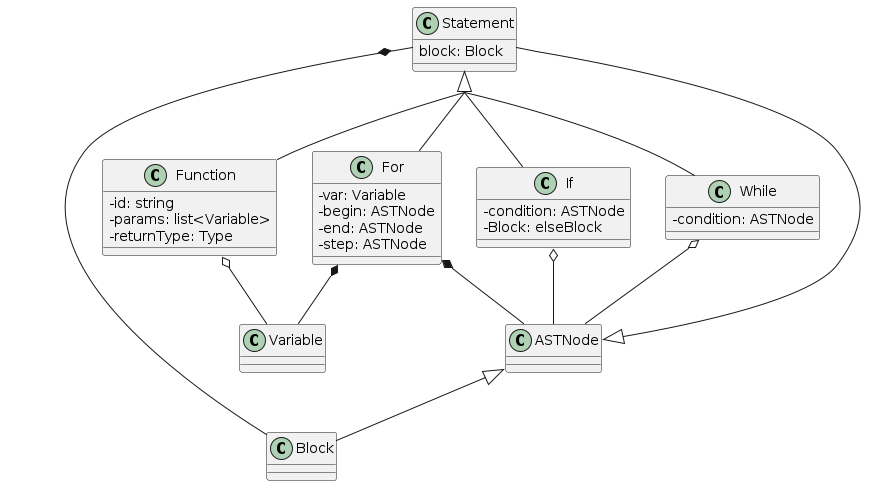
\includegraphics[scale=0.5]{../ressources/diagrams/stmts.png}
  \caption{Diagramme de classe: Statement}
  \end{center}
\end{figure}

De plus, on peut aussi voir sur ce diagramme la composition de la classe
\textit{Function} ainsi que celles des classes des structures de contrôle.

La classe \textit{Function} possède un attribut \textit{id} qui correspond au nom de la
fonction. Elle possède aussi un liste de variables qui sont ses paramètres ainsi
qu'un type de retour (le type \textit{Type} est détaillé plus loin).

La classe \textit{For} possède une variable qui est la variable de boucle et les
trois valeurs fournies par le \textit{range} décrites précédemment.

La classe \textit{If} possède un nœud qui contiendra l'opération booléenne de la
condition. Elle possède aussi un second \textit{Block} qui contient les
instructions du \textit{else} s'il y en a un.

Enfin la classe \textit{While} possède comme \textit{If}, un nœud pour la
condition.

\subsubsection*{Les opérations}

Les opérations sont traitées avec la classe \lstinline{OperationBinaire} qui
correspond à tous les opérateurs. Cette classe possède deux attributs de type
\textit{ASTNode} qui représentent les parties gauche et droite d'une opération
binaire. Pour ne pas trop alourdir le schéma ci-dessous, seul la classe
\textit{AddOP} a été représentée, cependant, toutes les fonctions décrites dans
partie \ref{sec:operator} ont une classe qui hérite de
\lstinline{OperationBinaire}.
\clearpage

\begin{figure}[h!]
  \begin{center}
  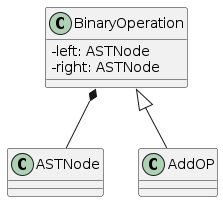
\includegraphics[scale=0.5]{../ressources/diagrams/binaryOp.png}
  \caption{Diagamme de classe: BinaryOperation}
  \end{center}
\end{figure}

\subsubsection*{Les éléments typés}
\label{sec:eltTypes}

Les fonctions, les valeurs et les variables possèdent un champ type. Le type
\textbf{Type} est une énumération qui possède les éléments visibles sur le
diagramme suivants :

\begin{figure}[h!]
  \begin{center}
  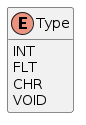
\includegraphics[scale=0.5]{../ressources/diagrams/Type.png}
  \caption{Enumération Type}
  \end{center}
\end{figure}

Le champ INT correspond au type des entiers, le champ FLT au type des flottants
et le champ CHR au type des caractères. Le type VOID est utilisé pour le type de
retour des procédures et il est aussi utilisé par le parseur pour créer des
variables qui n'ont pas été déclarées (car on ne plante pas dans ce cas).

\subsubsection*{Les valeurs}

Le dernier élément de l'AST que nous traiterons est la classe \lstinline{Value}
qui permet de représenter les valeurs utilisées dans le code. Comme on peut le
voir sur le diagramme ci-dessous, cette classe possède deux attributs,
\textit{type} qui représente le type de la valeur et \textit{value} qui permet
de stocker la valeur. Le type \textit{type\_t} est une union qui contient un
caractère, un entier et un flottant et permet donc de stocker des valeurs pour
ces trois types.

\begin{figure}[h!]
  \begin{center}
  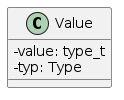
\includegraphics[scale=0.5]{../ressources/diagrams/value.png}
  \caption{Diagramme de classe: Value}
  \end{center}
\end{figure}
~\\

Nous avons défini la grammaire du langage et déterminé les différents éléments
qui vont composer notre arbre syntaxique. Dans la partie suivante nous écrirons
la grammaire décrite précédemment dans le langage de bison et nous montrerons
la construction d'un programme en utilisant les classes de l'AST que nous
venons de décrire.


\clearpage{}

\section{Construction de l'AST}

Dans cette partie nous expliquerons la création d'un parseur en utilisant les
outils \textbf{GNU Flex} et \textbf{GNU Bison}. De plus, nous détaillerons la
génération de l'AST en utilisant les classes décrites précédemment. Pour cette
partie, nous nous sommes aidés d'un article \cite{compilerFlexBison} qui
présente la construction d'un compilateur avec Flex et Bison en C. Pour porter
le code en C++, nous avons utilisé la documentation officielle des deux outils
ainsi qu'un article qui nous a permis d'avoir un squelette de base pour le
\gls{lexer} et le parseur \cite{cppparsing}.

\subsection{Le lexeur}

Pour faciliter le travail du parseur nous allons utiliser un lexeur. Dans
cette partie, nous détaillerons la conposition du fichier de configuration qui
nous permettra de générer le code du lexeur avec l'outil Flex. Nous verrons dans
la partie suivante comment utiliser les tokens dans les règles de grammaire.

\subsubsection*{Exemple}

Pour l'expression simple \textbf{a = 2 * b} \\
Les tokens apparaissant sont : \\
\begin{center}
  \begin{tabular}{ | c | c | }
    \hline
    \textbf{Token} & \textbf{Sa nature} \\
    \hline
    a & Identificateur de variable \\
    \hline
    = & Symbole d'affectation \\
    \hline
    2 & Valeur entière \\
    \hline
    * & Opérateur de multiplication \\
    \hline
    b & Identificateur de variable \\
    \hline
  \end{tabular}
\end{center}

Le lexeur a également pour rôle de supprimer les informations inutiles,
généralement des caractères blancs (espaces et tabulations) et des
commentaires.\\~\\

%\phantomsection
\subsubsection*{Implémentation}

Comme évoqué précédemment, l'outil utilisé pour générer le lexeur est
\textbf{GNU Flex} (Fast LEXical analyser generator). Il permet de générer le
code C++ du lexeur à partir d'un fichier. Dans notre cas, le fichier utilisé
sera \textbf{main\_cpp.l} et possède la structure suivante
\cite{compilerFlexBison} :

\begin{code}
// code C++, options et declarations de raccourcis

%%
// Definition des tokens et actions

%%
// Fonctions C++
\end{code}\leavevmode\newline

\noindent

Dans la première partie en haut du fichier, on place les inclusions de
bibliothèques C/C++ ainsi que des options pour Flex.

\begin{code}
%{
#include "parser.hpp"
#include "lexer.hpp"
%}

%option c++ interactive noyywrap yylineno nodefault outfile="lexer.cpp"
\end{code}\leavevmode\newline

Détail des fonctions utilisées :
\begin{itemize}
  \item \textbf{c++} : indique qu'on travail avec du cpp et non du c
  \item \textbf{interactive} : utile quand on utilise \textbf{std::in}. Le
    scanner interactif regarde plus de caractères avant de générer un token
    (plus lent mais permet de lutter contre les ambigüités)
  \item \textbf{noyywrap} : ne pas appeler \textbf{yywrap()} qui permet de
    parser plusieurs fichiers
  \item \textbf{nodefault} : pas de scanner par défaut (=> on doit tout
    implémenter)
  \item \textbf{outfile:"file.cpp"} : permet de définir le fichier de sortie
\end{itemize}\leavevmode\\

Après les options on peut définir des raccourcis en utilisant des expressions
régulières. Par exemple, dans le code ci-dessous, nous avons défini les règles
suivantes :

\begin{itemize}
  \item \textbf{alpha :} un caractère alphabétique est composé d'une lettre
    minuscule ou d'une lettre majuscule.
  \item \textbf{digit :} les chiffres sont les caractères entre 0 et 9.
  \item \textbf{int :} les entiers correspondent à une suite de chiffres et
    peuvent être positifs ou négatifs.
  \item \textbf{float :} similaire aux entiers sauf qu'ici on a obligatoirement
    un point suivi d'une suite de chiffre à la fin.
  \item \textbf{char :} les caractères sont toujours écrits entre \textbf{'}
    (par exemple \textbf{'a'}).
  \item \textbf{identifier :} correspond aux noms de fonctions et de variables
    et suit le standard du C. Un identifiant commence par une lettre minuscule
    et peut être suivi d'une suite de lettres, de nombres et de \textbf{\_}.
\end{itemize}

\begin{code}
alpha [a-zA-Z]
digit [0-9]
int [+-]?{digit}+
float [+-]?{digit}+\.{digit}+
char '{alpha}'
identifier [a-z]({alpha}|{digit}|_)*
\end{code}\leavevmode\newline

\noindent

On peut déjà noter que nous venons de définir l'identifiant qui correspond aux
noms des variables et fonctions et que cela correspond bien à ce qui a été
énoncé dans la grammaire.\\

Dans la seconde partie du fichier, on définit des règles et des actions. À noter
que l'on peut utiliser les raccourcis définis précédemment en mettant leurs noms
entre accolades comme fait ci-dessous pour \textbf{identifier}. La définition
d'une règle suit le principe suivant, on commence par donner une suite de
caractères qui sera consommée. Ensuite on ajoute du code entre accolades, qui
sera exécuté quand le lexeur consommera la chaine. Par exemple, si on prend la
première ligne ci-dessous, quand le lexeur trouvera le mot \textbf{for}, il
affichera \textit{L\_for} dans le terminal puis retournera le token \textbf{FOR}.

À noter que les tokens disponibles dans l'espace de nom \textbf{Parser::token}
doivent être définis dans le ficher Bison que l'on détaillera dans la partie
suivante.

\begin{code}
for          { AFFICHE("L_for"); return Parser::token::FOR; }
{identifier} {
  AFFICHE("L_id");
  yylval->build<std::string>(yytext);
  return Parser::token::IDENTIFIER;
}
\end{code}\leavevmode\newline

\noindent

Ici on a accès à la variable \textcolor{purple}{yylval} de type
\textcolor{purple}{Parser::semantic\_type*} qui possède une méthode
\textcolor{purple}{build} permettant de transmettre des valeurs à bison.\\

La fonction appelée par défaut est \textcolor{purple}{yylex}, cependant, pour
pouvoir travailler avec bison, nous devons fournir nos propres fonctions, pour
ce faire on utilise la macro \textcolor{purple}{YY\_DECL}, comme expliqué dans
la partie \textit{9 The Generated Scanner} du manuel pour Flex
\cite{flexmanual}.

\begin{code}
#define YY_DECL int interpreter::Scanner::lex(Parser::semantic_type *yylval, Parser::location_type *yylloc)
\end{code}\leavevmode\\~\\

Cette macro permet de définir le type de la fonction \textbf{lex}, ici,
on a pour paramètre \textcolor{purple}{yylval} (qui comme dit précédemment permet
de transmettre des valeurs à bison) et \textcolor{purple}{yylloc} qui doit être
fourni quand on utilise les positions dans le parseur (pour avoir le numéro de
ligne en cas d'erreur par exemple), mais cela nécessite une option particulière
pour bison.

\clearpage{}

\subsection{Le parseur}

Dans cette partie nous allons utiliser le travail précédemment effectué sur le
lexeur pour écrire des règles de grammaire. Nous détaillerons la
composition de ces règles et en quoi elles permettent la construction de notre
arbre syntaxique.

\subsubsection*{Exemple}

Pour l'expression simple \textbf{a = 2 * b} \\
On peut voir dans le tableau suivant l'analyse d'une affectation par le
parseur :\\
\begin{center}
\begin{tabular}{ | c | c | c | }
\hline
\textbf{Arbre syntaxique} & \textbf{Évaluation de 2 * b} & \textbf{Affectation de a} \\
\hline
\Tree[.= a  [.* 2 b ]] &
    \Tree[.= a  2*b ] &
        a = 2 * b\\
\hline
\end{tabular}
\end{center}

%\phantomsection
\subsubsection*{Implémentation}

À l'instar de Flex pour le lexeur, Bison est un générateur de grammaire qui
convertit une description de grammaire en un programme C++ qui analyse cette
même grammaire.\\

Le fichier \textbf{main\_cpp.y} contient le code qui permet de générer le
parseur avec Bison. Toutes les règles syntaxiques qui définissent la grammaire
du langage y sont comprises. Chaque règle va contenir des blocs de code qui
seront exécutés au moment où le parseur la reconnait, ce code permet de
construire l'AST du programme ainsi que de faire de la vérification sur les
symboles, comme nous le verrons plus tard.\\

La structure du fichier \textbf{main\_cpp.y} est similaire à celle du lexeur :

\begin{code}
// C++, options, et declaration des tokens

%%
// Regles de grammaire

%%
// fonctions C++
\end{code}\leavevmode\newline

Les tokens sont définis en début de fichier avec la syntaxe suivante:

\begin{code}
%token IF ELSE FOR WHILE FN INCLUDE IN
%token <long long>  INT
%token <double>     FLOAT
%token <char>       CHAR
%token <std::string> IDENTIFIER
\end{code}\leavevmode\newline

On peut aussi voir dans le code ci-dessus que certains tokens possèdent un type.
Cela permet de pouvoir récupérer les valeurs retournées par le lexeur. Il est
aussi possible de déclarer le type d'une règle de grammaire pour que celle-ci
puisse retourner une valeur comme nous le verrons plus loin.\\~\\


L'objectif de Bison est de pouvoir générer le code d'un parseur à partir des
règles définies dans le fichier. Voici un exemple de règle :

\begin{code}[language=c++]
function:
        FN IDENTIFIER[name]'('paramDeclarations')' block[ops]
        |
        FN IDENTIFIER[name]'('paramDeclarations')' ARROW type[rt] block[ops]
        ;
\end{code}\leavevmode\newline

Dans le code ci-dessus, on définit la règle pour les fonctions. La définition
d'une règle se fait de la façon suivant :

\begin{itemize}
  \item On donne le nom de la règle suivit de ':'.
  \item On décrit ensuite la règle en utilisant les tokens ou directement des
    caractères comme c'est le cas ci-dessus pour les parenthèses. On peut aussi
    utiliser les autre règles définies dans le fichier, par exemple, ici on
    utilise les paramètres, les blocs ainsi que les types.
  \item Le caratère \textbf{'|'} est utilisé lorsque la règle est composée de
    plusieurs sous règles. Dans le code ci-dessus, il y a deux sous règles pour
    les fonctions, une où on spécifie le type de retour et l'autre où on ne le
    spécifie pas. À noter que l'on ne peut pas ajouter d'éléments optionnels
    comme on pouvait le faire avec la forme de Backus-Naur entre \textbf{'[]'}.
    Dans ce cas il faut définir plusieurs sous règles.
\end{itemize}~\\

On peut ajouter des blocs de codes qui seront exécutés au moment où le parseur
atteint l'élément qui précède le bloc. Si on reprend l'exemple des fonctions on
obtient le code suivant :

\begin{code}[language=c++]
function:
        // premiere regle sans le type de retour
        |
        FN IDENTIFIER[name]'('paramDeclarations')' ARROW type[rt]
        {
          contextManager.newSymbol($name, $rt, FUNCTION);
          contextManager.enterScope();
        }
        block[ops]
        {
          pb.createFunction($name, $ops, $rt);
          contextManager.leaveScope();
        }
        ;
\end{code}\leavevmode\newline

Dans cet exemple on a ajouté deux blocs de code. Le premier sera exécuté juste
avant de rentrer dans le bloc d'instructions \textit{block} de la fonction. Le
second sera exécuté une fois que le bloc d'instructions aura été traité. On
peut voir que dans les blocs que nous venons d'ajouter, nous pouvont accéder
aux valeurs des différents éléments qui composent la règle. Par exemple,
\textcolor{purple}{\$name} permet d'accéder à la valeur de l'identifiant et de
la même façon, \textcolor{purple}{\$ops} permet de récupérer la valeur renvoyée
par la règle \textbf{block}. À noter qu'ici tous les éléments  auxquels on doit
accéder ont été nommés, cependant, il n'est pas obligatoire d'ajouter un nom
entre \textbf{'[]'}. S'il n'y a pas de nom, on utilise des nombres, par exemple,
s'il n'y avait pas \textbf{[name]} derrière \textbf{IDENTIFIER}, on aurait
utilisé \textcolor{purple}{\$1} car c'est le premier élément qui possède une
valeur (le token \textbf{FN} n'a pas de type et Flex ne retourne rien).\\


Comme dit plus haut, on peut définir une valeur de retour pour les règles, pour
ce faire, il faut définir un type à la règle, dans la première partie en haut du
fichier puis utiliser \textcolor{purple}{\$\$}. L'exemple ci-dessous correspond
à la règle pour les valeurs, dans ce cas on récupère la valeur retournée par
Flex, puis on "instancie" une nouvelle \textit{Value} qui est ensuite renvoyée.

\begin{code}[language=c++]
// en haut du fichier
%nterm <Value> value

%%
// regles

value:
     INT {
       type_t v = { .i = $1 };
       $$ = Value(v, INT);
     }
     |
     FLOAT {
       type_t v = { .f = $1 };
       $$ = Value(v, FLT);
     }
     |
     CHAR {
       type_t v = { .c = $1 };
       $$ = Value(v, CHR);
     }
     ;
\end{code}\leavevmode\newline

Pour la génération du code, on a deux options :
\begin{itemize}
  \item utiliser des instructions très simples (comme du bytecode)
\item créer un code objet où tous les éléments sont des objets.
\end{itemize}\leavevmode\\~\\

\underline{Choix de la représentation objet} :
\begin{itemize}
\item plus simple à comprendre et à visualiser
\item plus compliquée à générer: on peut générer du bytecode au fil de
  l'exécution du parseur, en utilisant des \textcolor{orange}{goto} pour
    sauter de bloc d'instructions en bloc d'instructions. Pour le code objet,
    les éléments à l'intérieur des blocs doivent être créés avant le bloc, et
    le bloc est détecté avant les instructions, il faut donc les stocker.
\end{itemize}


\clearpage{}

\subsection{Fabrique à programme}\label{sec:fabprog}

Pour construire l'arbre syntaxique dans le programme, nous utiliserons
la classe \textbf{ProgramBuilder}. Cette classe permet de stocker des éléments
comme le nom de la fonction courante ou les commandes récupérées par le
parseur.
De plus cette classe permet d'instancier les éléments de l'AST pour construire
le programme. Le diagramme de cette classe est le suivant :

\begin{figure}[h]
  \begin{center}
  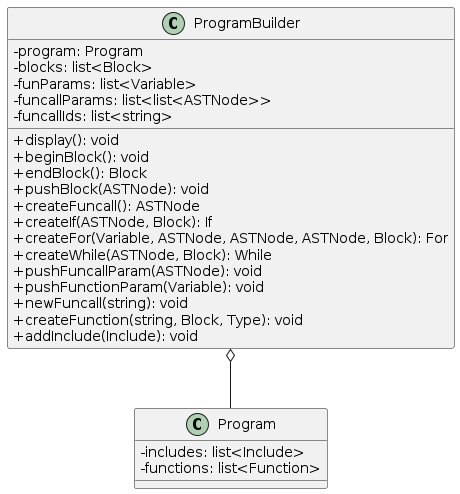
\includegraphics[scale=0.5]{../ressources/diagrams/program-builder.png}
  \caption{Diagramme de classe : ProgramBuilder}
  \end{center}
\end{figure}

On peut noter sur ce diagramme que l'on a des fonctions de créations qui
permettent de créer les éléments de l'AST définis dans la première partie. De
plus la classe est composée du programme, auquel elle ajoute les fonctions et les
fichiers inclus. % note: ça va changer

L'emploi de cette classe permet de limiter le code dans le parseur mais aussi de
pouvoir récupérer des éléments dans des piles quand on ne connait pas leur
nombre. Par exemple, pour les \textbf{Block}, on ne sait pas combien de
commandes ils contiennent, c'est pourquoi le \textbf{ProgramBuilder} possède une
pile qui permet d'ajouter les commandes aux blocs ainsi que d'avoir accès au
dernier bloc pour construire les \textbf{Statement}. Il en est de même pour
les paramètres de fonctions, dans ce cas nous avons une liste de listes. Si une
fonction \textbf{A} prend le résultat d'une autre fonction \textbf{B} en
paramètre (\textit{A(..., B(...), ...)}), la dernière liste contient les
paramètres de \textbf{B} au moment ou \textbf{B} est traitée. À l'origine, ce
choix avait été fait car il permet de toujours avoir accès aux éléments qui sont
en train d'être récupérés depuis n'importe quel endroit du parseur. Cependant,
cette fonctionnalité n'est pas utilisée, il aurait donc été plus simple de
construire ces listes en utilisant les valeurs de retour de bison.\\
% NOTE: je sais plus parler

Le \textbf{ProgramBuilder} permet donc de stocker les éléments importants ainsi
que de construire le \textbf{Program} au fur et à mesure de l'exécution du
parseur.


\section{Analyse des symboles}

Dans cette partie, nous allons créer une table des symboles qui, de façon
similaire à ce que l'on voit dans \cite{compilerFlexBison}, permet de vérifier
si les symboles (variables et fonctions) utilisés ont bien été déclarés.
Cependant, ici notre table des symboles sera plus complexe du fait que les
symboles peuvent avoir des portées différentes. De plus la table des symboles
nous permettra aussi de faire de la vérification de types pour par exemple,
vérifier qu'une fonction prend les bons paramètres.

Comme nous allons devoir faire de la détection d'erreurs, nous créerons une
nouvelle classe qui permettra de stocker tous les messages d'erreurs (et
avertissements) au fil de l'exécution du parseur. Ces messages seront affichés à
la fin une fois tout le code source traité. À noter que la présence d'erreurs
empêche la compilation.

\subsection{Gestion des symboles}

\subsubsection*{La table des symboles}

Pour la création de notre table des symboles nous utiliserons la méthode
présentée dans cet article \cite{power2000symbol} que nous avons simplifié pour
la récupération et la recherche de symboles.\\

Commençons par étudier la composition d'un symbole. Chaque symbole est composé
d'un nom qui lui sert d'identifiant, d'un type et d'un genre. Le genre est une
énumération qui suit le même principe que dans \cite{power2000symbol}. Le type
du symbole est une liste de \textbf{Type} qui est une énumération décrite dans
l'AST, il a la même utilité que pour les éléments typés (voir la section
\ref{sec:eltTypes}). Ici nous stockons une liste de \textit{Type} et non
juste un \textit{Type}. En effet le type d'une variable est bien composé d'un
seul \textit{Type} (une liste de un élément) mais le type des fonctions ne
correspond pas uniquement au type de la valeur de retour. Le type d'une fonction
comprend aussi le type de chacun des paramètres.

\begin{figure}[h!]
  \begin{center}
  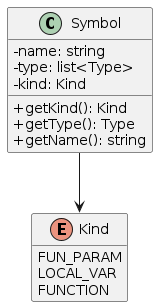
\includegraphics[scale=0.5]{../ressources/diagrams/symbol.png}
  \caption{Diagramme de classe : Symbol}
  \end{center}
\end{figure}

Pour implémenter la table des symboles nous nous sommes inspirés du schéma
suivant \cite{symtableGenius}. Ici la table des symboles est une table de
tables. Chaque sous table correspond à une zone de code dans laquelle peuvent
être définis des symboles (\textbf{scope}). Cette représentation est
intéressante car elle permet de pouvoir aisément vérifier si un symbole existe
en remontant l'arborescence de la table jusqu'au \textbf{scope} global. Les
éléments stockés dans la table mère sont toujours accessibles.
\clearpage

\begin{figure}[h!]
  \begin{center}
  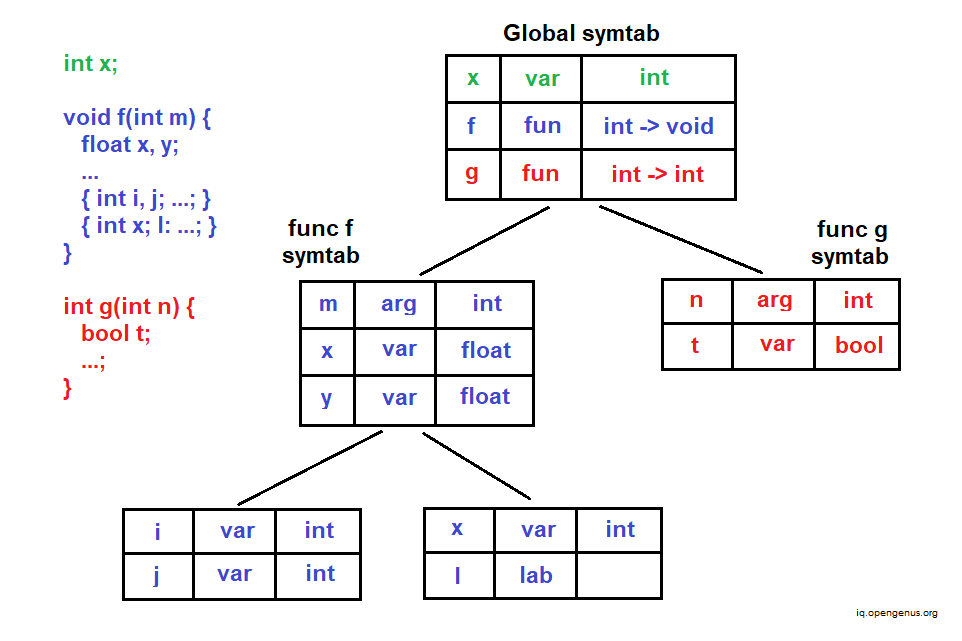
\includegraphics[scale=0.5]{./img/symtable.png}
  \caption{Structure de la table des symboles}
  \end{center}
\end{figure}

Pour l'implémentation, nous suivrons le diagramme ci-dessous. Les symboles sont
stockés dans une \textbf{unordered\_map} qui est une table de hachage qui
permettra l'accès aux valeurs avec l'identifiant. De plus, la table
possède une liste de sous tables qui est un pointeur sur la table mère qui sera
utilisé par la méthode \textbf{lookup} pour la recherche de symbole comme
expliqué précédemment. À noter que la méthode \textbf{lookup} ne renvoie pas
directement un symbole. Elle utilise la classe \lstinline{std::optional} et
renvoie une valeur vide dans le cas où le symbole recherché n'a pas été trouvé,
ce qui est pratique étant donné le fait que C++ ne possède pas de valeur nulle.
Une autre solution aurait été de retourner un pointeur.

\begin{figure}[h!]
  \begin{center}
  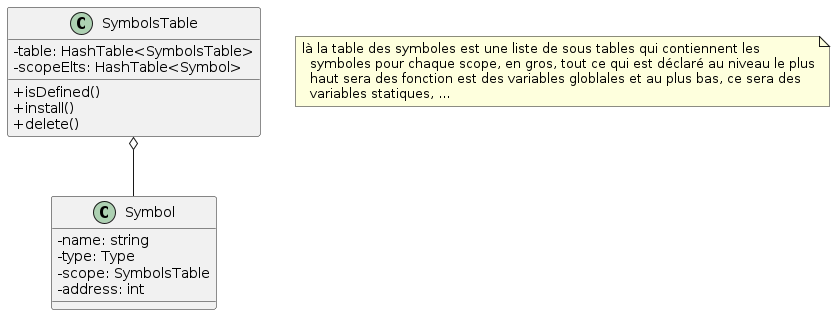
\includegraphics[scale=0.5]{../ressources/diagrams/symtable2.png}
  \caption{Diagramme de classe : Symtable}
  \end{center}
\end{figure}

Nous avons donc une table des symboles qui nous permet de connaître tous les
éléments nommés du programme, leur portée ainsi que leur type. Dans la partie
suivante, nous détaillerons le fonctionnement de l'objet responsable de la
création de la table dans le parseur.

\clearpage
\subsubsection*{Gestion du contexte}

Nous avons une table des symboles, cependant il nous faut un moyen de gérer les
\textit{scopes}, et donc de gérer l'arborescence de la table. Pour ce faire nous
aurons une classe \textbf{ContextManager} qui permettra de créer des nouveaux
nœuds dans l'arborescence de la table des symboles à chaque fois que l'on entre
dans un nouveau \textit{scope}. La structure de cette classe est la suivante :

\begin{figure}[h!]
  \begin{center}
  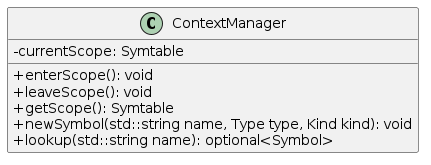
\includegraphics[scale=0.5]{../ressources/diagrams/contextManager.png}
  \caption{Diagramme de classe : ContextManager}
  \end{center}
\end{figure}

Le \textbf{ContextManager} possède un attribut \textbf{currentScope} qui est pointeur sur
la sous table qui contient le scope courant. La classe possède aussi deux
méthodes permettant de rentrer ou sortir d'un scope. La méthode
\textbf{enterScope} crée une nouvelle sous table dans la table des symboles et
pointe dessus avec \textbf{currentScope}. Lorsqu'on sort du scope courant, on
retourne dans le \textit{scope père}, la méthode va donc faire pointer
\textbf{currentScope} sur la table mère. Enfin cette classe possède des méthodes
pour ajouter ou rechercher des symboles qui font appel aux méthodes de la sous
table courante.\\

Le \textbf{ContextManager} permet donc de créer une table des symboles dans le
parseur, ainsi que de pouvoir faire toutes les vérifications décrites dans la
partie précédente. La partie suivante concerne la création d'une classe pour la
gestion des erreurs de compilation. Nous verrons ensuite comment combiner toutes
ces classes dans le parseur pour pouvoir collecter et afficher toutes les
erreurs de types et de définitions.

\subsection{Gestion des erreurs}

L'objectif de cette partie est de pouvoir vérifier si les éléments du programme
ont bien été définis et possèdent les bons types. Dans le cas contraire, cela va
impliquer de devoir renvoyer les bonnes erreurs. Pour ce faire, nous avons une
classe dédiée à la collections des erreurs et des avertissements dans le
parseur, \lstinline{ErrorManager}.

Comme on peut le voir ci-dessous sur le diagramme, c'est une classe très simple
qui ne possède que deux attributs. Le premier est un flux de caractères qui va
permettre de stocker tous les messages d'erreurs. Le second est un booleen, il
est initialisé à \textit{false} au départ et passe à \textit{true} quand une
erreur est enregistrée. Cet attribut sert à savoir si on doit compiler ou pas
quand le parseur a consommé tout le texte. En effet, seules les erreurs de
syntaxes sont bloquantes, et causent un arrêt du parseur avec un retour non nul.
Cependant, il n'est pas nécessaire de planter au niveau du parseur pour les
erreurs de types. De ce fait il nous est possible de récupérer toutes les
erreurs de type dans un programme qui ne comporte pas d'erreur de syntaxe et
donc de rendre la correction du programme plus rapide.

\clearpage
\begin{figure}[h!]
  \begin{center}
  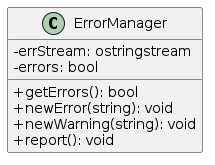
\includegraphics[scale=0.5]{../ressources/diagrams/errMgr.png}
  \caption{Diagramme de classe : ErrorsManager}
  \end{center}
\end{figure}

Concernant les méthodes, la classe possède une méthode \textit{report} qui doit
être appelée après le parseur et affiche tous les messages enregistrés. La
classe possède aussi deux méthodes permettant l'ajout de nouvelles erreurs et
de nouveaux avertissements. La différence entre les deux est que les
avertissements ne vont pas empêcher la transpilation. Par exemple, un
avertissement peut être levé lors de l'affectation d'un caractère à une variable
de type entier. Ici, l'avertissement va permettre de signifier à l'utilisateur
que les types diffèrent, cependant, ce dernier souhaite peut-être extraire le
numéro ASCII du caractère assigné, il ne faut donc pas planter dans ce genre de
cas.\\~\\

\subsection{Traitement des symboles dans le parseur}

Dans cette partie, nous allons utiliser les composants implémentés précédemment
pour les intégrer dans le parseur. Nous allons donc modifier les blocs de
codes dans le fichier bison pour faire des vérifications lorsque c'est
nécessaire.

\subsubsection*{Vérification des définitions}\label{sec:verifDef}

Ici, notre objectif va être de vérifier que toutes les variables utilisées dans
le code ont été déclarées au préalable. Nous vérifierons aussi que toutes les
fonctions appelées dans le programme ont été définies. Enfin, il faudra aussi
s'assurer de la définition d'une fonction \textit{main}. En effet, de façon
similaire au C, la grammaire de notre langage n'autorise pas l'ajout
d'instructions à l'extérieur des fonctions. De ce fait, tout programme doit
avoir un point d'entrée.\\

Pour faire les vérifications, nous avons implémenté diverses fonctions. La
première fonction \textit{isDefined} prend en entrée un nom, les numéros de
ligne et de colonne ainsi qu'une référence sur une liste de \textit{Type}.
Cette fonction renvoie vrai lorsque le symbole demandé (le nom) est défini et
elle modifie le type par effet de bord. De ce fait, on peut accéder facilement
au type dans les blocs de code du parseur. La fonction se charge aussi
de générer une erreur en utilisant les numéros de ligne et de colonne pour
indiquer la position de l'erreur.

Nous avons aussi une fonction qui permet de vérifier le type des paramètres lors
d'un appel de fonction. Celle-ci n'utilise pas directement la table des
symboles, elle prend en paramètre deux listes qu'elle compare et renvoie un
booléen en fonction du résultat.

Une seconde fonction de vérification de type à été écrite, mais celle-ci génère
un avertissement et non une erreur. Elle est utilisée au niveau de l'affectation
pour ne pas générer d'erreur lorsque l'on fait de la conversion de type comme
expliqué précédemment.

Enfin on a une fonction \textit{getType} qui permet de récupérer le type de la
valeur d'un symbole (uniquement le type de retour s'il s'agit d'une fonction).

À noter que cette partie n'est pas idéale mais n'a pas pu être modifiée à cause
des contraintes de temps. Nous détaillerons le problème que nous avons ici ainsi
qu'une solution dans la partie discussion.\\

La vérification des définitions se fait à différents endroits. Tout d'abord elle
se fait au niveau de la règle de l'affectation pour vérifier si la variable à
qui on affecte une valeur a bien été déclarée. Ici on utilise bien la fonction
\textit{isDefined} qui génère un message d'erreur expliquant à l'utilisateur
qu'il tente d'affecter une valeur à une variable non définie. On fait aussi une
vérification au niveau de la règle qui permet de récupérer tous les éléments qui
peuvent avoir une valeur. Ici, on peut avoir des fonctions comme des variables.
La vérification se fait au niveau de la sous règle composée uniquement d'un
\textit{IDENTIFIER}, car on ne souhaite pas faire la vérification sur des
\textit{Value} ou des opérations arithmétiques.

Pour les fonctions, la vérification est faite au niveau de la règle qui décrit
les appels de fonctions. Comme nous l'avons expliqué, \textit{isDefined} se
charge aussi de récupérer le type de la fonction appelée. Nous détaillerons dans
la partie suivante la vérification du type.

À noter que comme les symboles sont récupérés et testés en même temps que le
parseur construit l'arbre, la collection des symboles suis le sens du texte. De
ce fait, toute fonction utilisée doit être définie au dessus de la fonction dans
laquelle elle est appelée. Cela peut être un problème car notre grammaire ne
permet pas la déclaration de fonctions, de ce fait il est pour l'instant
impossible d'avoir deux fonctions qui s'appellent entre elles sans avoir
d'erreur.\\

La vérification de la définition de la fonction \textit{main} se fait en
dernier, juste avant de transpiler. Nous savons que quand le parseur a fini de
tourner le \textit{ContextManager} est retourné au \textit{scope} global. Il
suffit donc de vérifier que la méthode \textit{lookup} retourne bien une valeur
lorsque l'on fait une recherche du symbole \textit{"main"}. À noter que du fait
que la grammaire n'autorise pas de variable globale, il ne peut y avoir qu'un
seul symbole nommé \textit{main} dans le \textit{scope} global, et celui-ci
correspond forcément à une fonction. Il n'est donc pas nécessaire d'utiliser
l'attribut \textit{Kind}, cependant, si l'on souhaitait ajouter des variables
globales, il faudrait faire plus de vérifications. De plus, nous n'avons pas
implémenté la possibilité de donner des arguments au programme, ce n'est donc
pas géré dans cette partie.

\subsubsection*{Vérification des types}

La seconde vérification à faire concerne les types des éléments. Pour la
récupération des types nous utiliserons certaines des fonctions décrites dans la
partie précédente.\\

Tout d'abord on fait une vérification de type au niveau de l'affectation.
Ici, on compare le type de la variable avec le type de la valeur affectée. On
utilise bien la fonction qui génère un avertissement et non une erreur pour la
conversion de type. La récupération du type se fait avec \textit{isDefined}
pour la variable et pour la valeur on utilise la fonction \textit{getType}
décrite plus haut.\\

C'est pour les fonctions que la vérification du type est complexe. Comme dit
précédemment, le type des fonctions comprend aussi leurs paramètres. La
vérification se fait en deux phases. Au niveau des appels de fonctions, on va
simplement vérifier le type de chacun des paramètres sans prendre en compte le
type de retour. Par contre, lorsque la fonction est traitée comme une valeur, on
ne regarde que le type de retour. Par exemple, si on regarde le code ci-dessous.

\begin{grammar}[language=C++]
  fonction1(a, 1, fonction2(3, 3));
\end{grammar}\leavevmode\newline

Dans cet exemple, on souhaite vérifier le type de \textit{fonction1}. Ici,
c'est un appel de fonction, on va donc vérifier les paramètres. Lors de cette
vérification, \textit{fonction2} sera traitée comme une valeur, on va donc
comparer le type de la valeur de retour de \textit{fonction2} avec celui du
dernier paramètre de \textit{fonction1}. À noter que la vérification des
paramètres de \textit{fonction2} a été faite au moment où l'appel de fonction a
été créé, donc avant la vérification de \textit{fonction1}.\\

Par manque de temps, la conversion des types au niveau des appels de fonctions
ne sera pas prise en charge. De ce fait, si une fonction prend en entrée un
entier, il faudra obligatoirement lui donner une variable ou une valeur de type
entier en paramètre pour ne pas avoir d'erreur. La conversion de type au niveau
des variables peut cependant se faire avec la fonction \textit{set}, le manque
de cette fonctionnalité n'est donc pas un problème.\\

Une dernière vérification de type est faite au niveau de la règle du
\textit{return}. Ici, on récupère le type de la fonction courante et on le
compare avec le type de la valeur renvoyée. Si les types ne correspondent pas,
une erreur est générée.\\

Nous avons décrit la construction de l'arbre syntaxique du langage et expliqué
la vérification des définitions et des types. De ce fait, nous somme capable de
donner un sens au code source ainsi que de vérifier qu'il est correcte. La
dernière étape concerne donc la traduction de l'arbre en python, ce qui fait
l'objet de la partie suivante.

\clearpage
\section{Le transpileur}

Dans cette partie, nous allons utiliser l'arbre syntaxique construit dans les
parties précédentes pour générer du code python. Pour la réalisation de cette
partie, nous n'avons pas eu le temps d'implémenter la solution que nous
souhaitions au départ. Cependant nous avons utilisé une solution temporaire
plus simple pour vérifier que nous étions bien capables de générer du code
correct en python. De plus, les éléments de notre transpileur actuel peuvent
être réutilisés pour réécrire le transpileur de façon plus propre.

\subsection{La solution idéale}

Comme on peut le voir dans cet article \cite{tutotranspiler}, une bonne solution
aurait nécessité la génération d'un second arbre syntaxique correspondant à la
syntaxe de python. En effet, le principe du transpileur et de faire une
traduction d'un langage vers un autre, cependant, la syntaxe et les
fonctionnalités du langage de départ peuvent être très différentes de celui
d'arrivée. Cela implique que certains éléments du langage source deviennent
impossibles à traduire dans le langage cible. Par exemple, si le langage source
est un langage fonctionnel, toutes les boucles doivent être remplacées par des
fonctions récursives. Si nous souhaitons transpiler ce type de langage en python
il faudra obligatoirement supprimer la récursivité car python limite le
nombre de fois qu'une fonction peut s'appeler elle-même (en plus du fait que
cela soit très lent). Dans ce cas extrême il y aurait beaucoup de modifications
à faire et il faudrait dérécursifier toutes les fonctions de l'AST d'origine
pour créer l'AST de python.

\subsection{Notre solution}

Par manque de temps, nous avons dû improviser une solution qui n'utilise pas de
deuxième arbre syntaxique. Nous avons donc décidé de directement faire la
traduction de notre arbre en python. Cela est possible car en l'état, notre
langage est très simple et ne possède pas de fonctionnalité que l'on ne peut pas
directement réécrire en python. Cela pourra cependant poser beaucoup de
problèmes si nous décidons d'ajouter de nouveaux éléments à notre langage ou
encore si nous souhaitons changer le langage cible pour du C par exemple.\\

Pour faire notre traduction, nous avons ajouté une méthode abstraite
\textit{compile} à la classe \textit{ASTNode}. Cette méthode est implémentée par
tous les éléments du langage. La méthode prend deux paramètres, le premier est un
flux \lstinline{std::ofstream} qui permet d'écrire dans le fichier de sortie. Le
second paramètre est un entier qui permet de connaitre le nombre de tabulations
à écrire pour indenter le code car python fonctionne avec l'indentation. Ce
nombre est incrémenté à chaque fois que l'on entre dans un bloc de code. La
traduction est lancée par le \textit{ProgramBuilder} qui appelle la méthode
\textit{compile} de toutes les fonctions du programme. À noter que le
\textit{ProgramBuilder} insère aussi un \gls{shebang} en haut du fichier pour
pouvoir exécuter le programme comme un exécutable classique sur les systèmes
UNIX. Cela nécessite aussi d'ajouter les droits d'exécutions au fichier ce qui
est fait dans la fonction \textit{main} après la traduction à l'aide de
\lstinline{std::filesystem::permissions}.

\section{Déroulement du projet}

\subsection{Les outils utilisés}

\subsubsection{Gestion de version}

Pour la gestion de version nous avons utilisé \textbf{git}, avec un dépôt
distant stocké sur github pour faciliter le partage du code. L'utilisation de
git permet d'avoir un suivi des modifications ce qui est utile lorsqu'une
mauvaise modification entraine de grosses erreurs. Le système de branche de git
permet aussi d'avoir un suivi des fonctionnalités et de pouvoir facilement
travailler à plusieurs. Cependant, du fait de la petite taille du projet et du
faible nombre de personnes dans le groupe, nous n'avons pas eu besoin de mettre
en place une méthode tel que gitFlow. Nous n'avons pas non plus eu le temps de
mettre en place des tests automatisés bien que cela aurait pu être nécessaire
sur la fin du projet pour tester le code python généré avec le transpileur. Une
suite au projet nécessitera certainement la mise en place d'une telle structure
de tests.\\

\subsubsection{Compilation}

Pour compiler le programme, nous avons au départ utilisé un \textit{Makefile}.
Cependant, nous avons basculé sur \textit{cmake} au moment de la création de la
table des symboles. Cmake permet de générer un \textit{Makefile} très complet à
partir d'un fichier de configuration. Un des avantages est que le fichier de
configuration de \textit{cmake} est moins verbeux que \textit{Makefile} car il
automatise la gestion des bibliothèques, des dépendances ainsi que des fichiers
objets. De plus le langage de \textit{cmake} permet beaucoup de choses comme par
exemple la possibilité de faire des conditions et des boucles. Cependant nous
n'avons pas utilisé ces fonctionnalités. Nous avons tout de même utilisé l'ajout
de cibles personnalisées pour la génération du lexeur et du parseur avec les
commandes \textbf{flex} et \textbf{bison}.

\subsection{Les recherches}

Pour les recherches, nous avons commencé par faire des recherches globales sur
le sujet pour avoir une idée du plan à suivre. Ces recherches nous on permis de
déterminer les éléments dont nous avions besoin pour créer le langage. La suite
des recherches s'est fait pendant l'implémentation des différents composants. Le
but était d'effectuer des recherches plus précises sur le composant à
implémenter pour prendre connaissance des différentes solutions et choisir
celle que nous jugions la plus intéressante. Pour faire nos recherches, nous
avons surtout utiliser \textit{google scholar} qui nous avait été recommandé
pour avoir des documents scientifiques certifiés. Nous avons aussi utilisé la
base de données \textit{technique de l'ingénieur} qui nous avait été présentée
lors de la séance sur la recherche documentaire. C'est sur cette base que nous
avons trouvé l'article concernant les compilateurs \cite{compilerTICH} qui nous
a permis de commencer le projet. Enfin, pour certains points nous avons aussi
utilisé \textit{google}, qui nous a notamment permis de trouver le tutoriel sur
la mise en place de Flex et Bison en C++ \cite{cppparsing}.

Trouver de bons documents n'a pas été simple, par exemple, nous avons essayé
d'utiliser la base \textit{ENI} mais les articles proposés ne nous ont pas aidé.

\clearpage
\subsection{Planification des tâches}

Dans cette partie, nous allons voir comment les différentes tâches on été
réalisées. Nous détaillerons deux diagrammes de Gantt, le premier correspondant
à la planification que nous pensions avoir en début de projet et le second à la
planification réelle. Ces deux diagrammes sont extrêmement différents, en effet,
nous étions au départ parti pour implémenter les différents composants les uns
après les autres. Cependant, nos premières recherches nous ont apporté presque
autant de questions que de réponses, nous sommes donc partis sur une méthode plus
itérative. Nous avons commencé par implémenter les composants dont nous étions
sûrs de l'utilité et du fonctionnement, pour avoir quelque chose de fonctionnel
qui nous permette de faire des tests. La correction d'erreurs à donc été
relativement simple étant donné que nous n'ajoutions que très peu de
fonctionnalités à chaque fois. Cependant, nous avons eu beaucoup d'hésitations
quand à nos choix d'implémentation et certaines parties du code ont été
réécrites plusieurs fois.\\

On peut donc voir sur ce premier diagramme que nous contions développer les
éléments les uns après les autres. Nous contions commencer par l'AST puis
implémenter le parseur, la table des symboles et le transpileur. À noter que
nous n'avions pas encore prévue de créer un objet pour la gestion des erreurs.
Ce diagramme est disponible en index \ref{appendix:expectedgantt} pour plus de
lisibilité.

\begin{figure}[h!]
  \begin{center}
  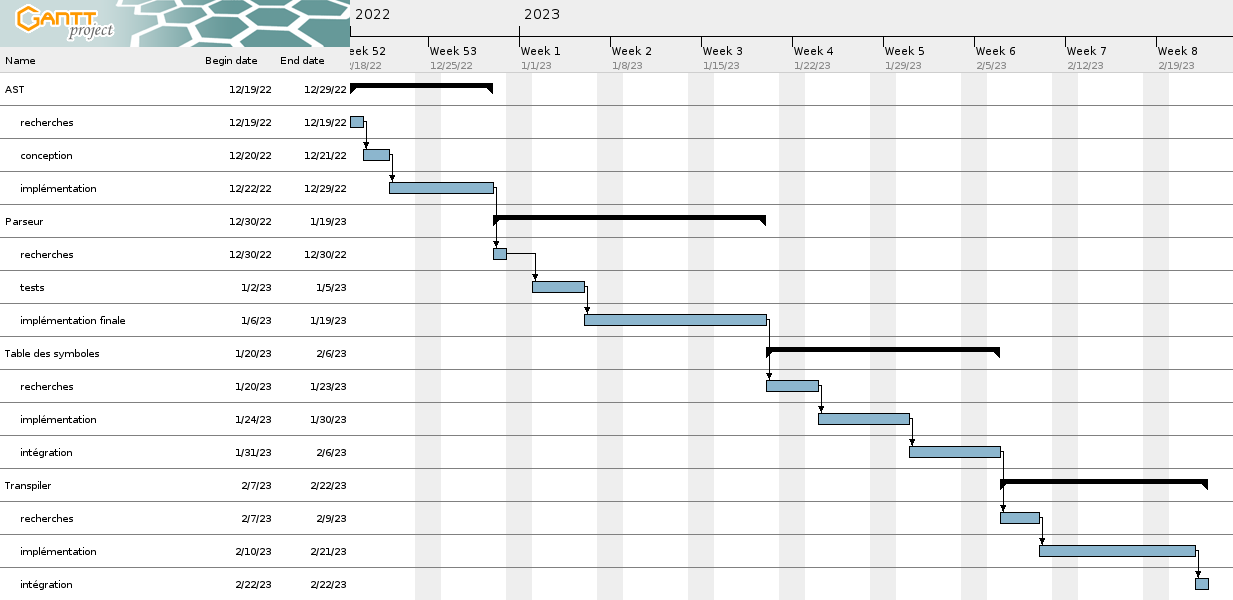
\includegraphics[scale=0.35]{./img/expected-gantt.png}
  \caption{Diagramme de Gantt prévisionnel}
  \end{center}
\end{figure}

Sur le diagramme réel, on peut constater que nous n'avons pas suivi le plan que
nous avions défini pour les raisons expliquées plus haut. Cependant, on peut
tout même voir que la table des symboles et le transpileur sont toujours fait
séparément du reste. Si on observe les trois premières parties, on peut voir
qu'elles correspondent à l'implémentation de l'AST et du parseur. De plus, si on
compare la durée, on peut constater que la conception de ces deux premiers
éléments a pris beaucoup plus de temps que nous l'avions prévu à cause de nos
hésitations. Pour la table des symboles, la durée globale a été assez bien
respectée. Si on regarde dans le détail on voit que l'implémentation a été plus
rapide que prévu mais nous avons dû implémenter la gestion d'erreurs en plus.
On peut enfin constater qu'étant donné le fait que les deux premières parties
ont été plus longues, le temps consacré à l'implémentation du transpileur a été
fortement réduit. Cela explique le fait que nous n'avons pas pu implémenter la
solution idéale. On peut aussi constater que les dates de fin diffèrent très
légèrement car nous avons finalement souhaité garder plus de temps pour
l'écriture de ce rapport. On peut retrouver ce diagramme en index
\ref{appendix:realgantt}.

\begin{figure}[h!]
  \begin{center}
  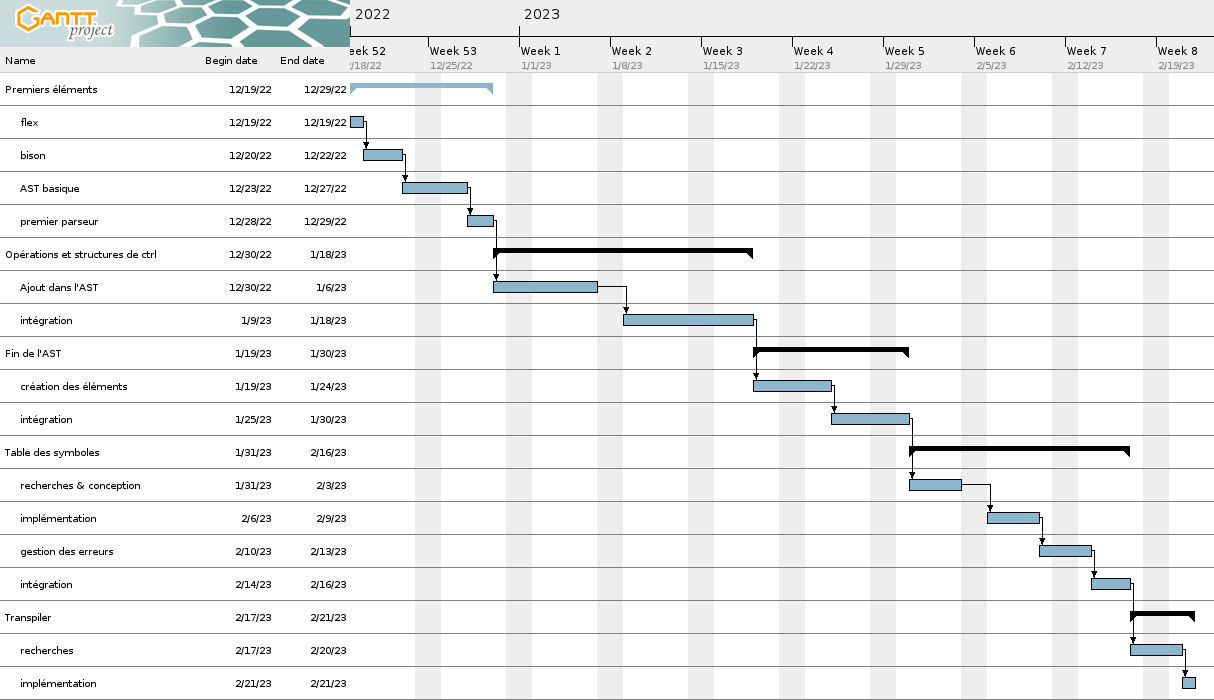
\includegraphics[scale=0.35]{./img/real-project.png}
  \caption{Diagramme de Gantt réel.}
  \end{center}
\end{figure}~\\

Nous avons donc traité le déroulement du projet dans cette partie. Dans la
dernière partie, nous présenterons les résultats obtenus et nous discuterons des
potentielles perspectives du projet.

\clearpage
\part{Résultats et discussions}

Dans cette partie, nous allons dans un premier temps présenter et critiquer les
résultats obtenus à la fin du projet. Nous parlerons aussi des améliorations et
corrections qui peuvent être apportées. Enfin, nous discuterons des perspectives
du projet.

\section{Fonctionnement du langage}

\subsection{La grammaire et les éléments du langages}

Au départ, les objectifs étaient de pouvoir créer des fonctions, des variables
typées et pouvoir faire des opérations arithmétiques et booléennes. Nous
souhaitions aussi avoir les structures de contrôle présentes dans la plupart des
langages. Au final, la grammaire du langage permet bien de faire tous ce que
nous souhaitions au départ. Cependant, comme nous l'avons évoquée dans la partie
\ref{sec:verifDef} notre grammaire ne pas permet à deux fonctions de s'appeler
entre elles. Cela vient du fait que nous n'avons pas créé de règle pour la
déclaration de fonctions comme ce que l'on peut avoir en C par exemple. Pour
palier à ce problème, nous pourrions ajouter une nouvelle règle de grammaire
pour déclarer les fonctions et ainsi créer les symboles correspondant avant de
traiter la définition.\\

Pour ce qui est du langage en lui-même, il aurait été intéressant de pouvoir
permettre la création de tableaux en plus de ce que nous avons fait. En effet,
pour l'instant la seule façon de stocker des données est d'utiliser des
variables ce qui n'est pas toujours idéal. Par exemple, l'ajout de tableaux
aurait permis la création de chaînes de caractères.\\

Le langage possède tout de même quelques fonctionnalités, et permet de coder la
plupart des algorithmes simples.

\subsection{Récupération des éléments du code}

En ce qui concerne le parseur, la prise en main de flex et bison a nécessité un
peu de temps. Comme expliqué dans la partie \ref{sec:fabprog}, nous aurions pu
plus utiliser les valeurs de retour de bison, ce qui aurait rendu le code plus
clair et plus intuitif. Ici, l'emploi du \textit{ProgramBuilder} est assez
complexe, et la classe fait énormément de choses ce qui n'est pas l'idéal.\\

On peut aussi constater que les règles de grammaire ont été assez bien définies
puisqu'il n'y a pas de répétitions. De plus, nous sommes bien capables de parser
tous les éléments que nous voulions intégrer au langage et de créer l'arbre
syntaxique qui convient.

\subsection{Gestion des erreurs}

Pour la gestion des erreurs nous avons pu faire des vérifications au niveau des
définitions et des types. Cependant, comme vu précédemment, les fonctions
employées pour l'accès à la table des symboles ne sont pas idéales. Il faudrait
donc refaire ces fonctions utilitaires et peut-être les intégrer au
\textit{ContextManager}.\\

Un autre point qui devrait être amélioré serait la gestion des erreurs de
syntaxe. En effet, pour l'instant, ce type d'erreur est uniquement géré par
Bison, qui s'arrête à la moindre erreur de syntaxe. Il est possible d'utiliser
une règle \textit{error} et une option \textit{yyerrok} pour éviter que le
parseur s'arrête sur certaines erreurs. Ce système n'est pas facile à utiliser
mais il pourrait servir à ne pas stopper le parseur en cas d'oublis de
\textbf{';'} à la fin d'une instruction par exemple. Il serait donc intéressant
d'améliorer la précision des erreurs de syntaxe, en donnant plus d'indications à
l'utilisateur et d'ajouter le fait que toutes ces erreurs ne font pas planter le
parseur.\\

Le dernier point d'amélioration concerne la localisation des erreurs. Pour
l'instant, nos messages d'erreurs donnent bien le bon numéro de ligne en
revanche nous n'avons pas réussi à faire fonctionner les numéros de colonne. Il
aurait aussi été intéressant d'afficher la ligne du programme qui comporte une
erreur comme le fait \textbf{gcc} par exemple.\\

\subsubsection*{Exemple}

On peut voir sur les deux figures ci-dessous l'affichage des erreurs sur un
programme test.

\begin{figure}[h]
  \begin{center}
  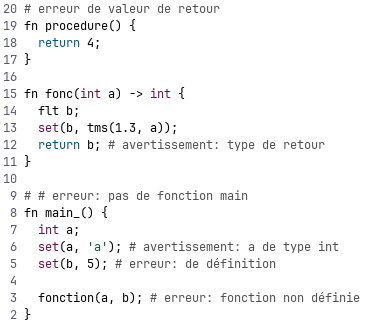
\includegraphics[scale=0.7]{./img/err-prog.png}
  \caption{Programme comportant des erreurs.}
  \end{center}
\end{figure}

\clearpage
On peut voir sur la figure que le programme affiche bien toutes les erreurs et
avertissements prévus. On peut aussi voir que la récupération des numéros de
colonne n'est pas fonctionnel et qu'il est toujours à 1.

\begin{figure}[h]
  \begin{center}
  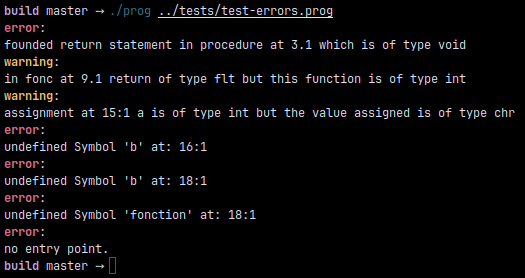
\includegraphics[scale=0.7]{./img/err-prog-out.png}
  \caption{Affichage des erreurs et avertissements.}
  \end{center}
\end{figure}

\subsection{Le transpileur}

Le transpileur n'a au final pas été fait de façon convenable, cependant nous
avons pu implémenter une solution qui nous permet de tester la génération de
code python. Notre solution fonctionne car le langage est très simple mais il y
a tout de même des problèmes. Le premier gros problème est le fait que les
classes de l'AST de notre langage se chargent de la traduction. Il aurait été
préférable que les classes de l'arbre n'aient aucun lien avec le transpileur. En
effet, si nous souhaitions changer le langage cible pour la traduction, ou
encore remplacer le transpileur par un compilateur, il faudrait modifier l'AST
ce qui ne devrait pas être le cas. De plus, comme nous l'avons dit, si nous
souhaitions ajouter de nouvelles fonctionnalités au langage cela pourrait
entrainer beaucoup de problèmes.

Enfin, bien qu'il soit très simple, le langage possède tout de même une
fonctionnalité qui n'est pas directement traduisible en python. En effet notre
langage possède un opérateur \textit{XOR}, ce qui n'est pas le cas de python.
Cela nous force à remplacer \textit{XOR(a, b)} directement par \textit{(a and
(not b)) or ((not a) and b)}. C'est un problème pour l'optimisation car les
expressions \textbf{a} et \textbf{b} sont évaluées plusieurs fois. Ici une
modification de l'arbre aurait permis de créer deux variables avant la condition
pour stocker les résultats des évaluations de \textbf{a} et \textbf{b}.\\

Bien que ça ne soit pas idéal, notre solution nous a tout de même permis de
tester notre langage pour différents programmes.\\

\clearpage
\subsubsection*{Exemple}

Voici un exemple simple de la fonction de fibonacci codée avec notre langage.
Comme le on peut le voir sur la figure ci-dessous, le programme demmande un
nombre à l'utilisateur, puis calcul et affiche le résultat de la fonction de
fibonacci sur ce nombre.

\begin{figure}[h]
  \begin{center}
  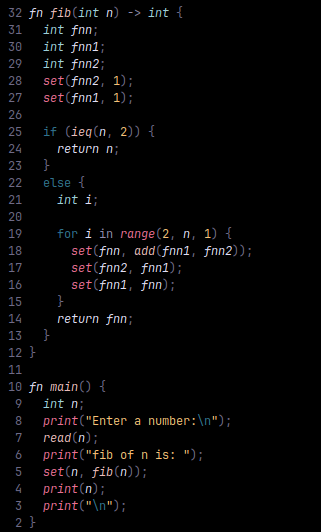
\includegraphics[scale=0.7]{./img/fib-prog.png}
  \caption{Test : fonction de fibonacci}
  \end{center}
\end{figure}

Sur la figure ci-dessous, on peut voir le résultat lorsqu'on entre la valeur 8.
On peut aussi constater que le programme compile sans erreurs.

\begin{figure}[h]
  \begin{center}
  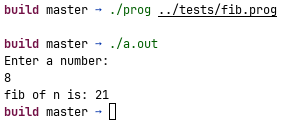
\includegraphics[scale=0.7]{./img/fib-prog-out.png}
  \caption{Affichage : fonction de fibonacci}
  \end{center}
\end{figure}

\clearpage
Voici le code python généré par le transpileur:

\begin{figure}[h]
  \begin{center}
  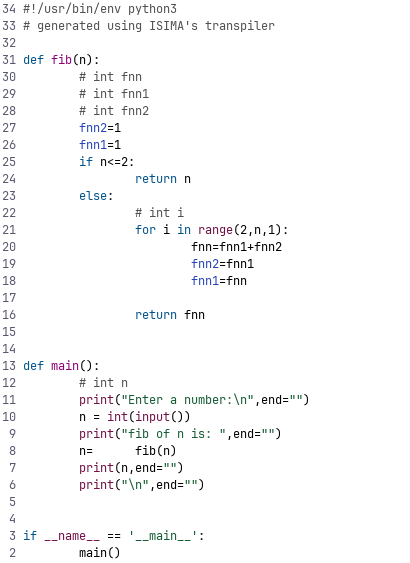
\includegraphics[scale=0.7]{./img/fib-prog-code.png}
  \caption{Code de fibonacci en python}
  \end{center}
\end{figure}

Dans le code ci-dessus, on peut remarquer plusieurs choses. Tout d'abord, comme
c'est à l'utilisateur de mettre les retours à la ligne lors des affichages, on
peut voir que l'on supprime le retour à la ligne automatique dans les
\textit{print} de python. De plus, on peut aussi remarquer la la valeur entrée
avec \textit{input} est modifiée pour correspondre au type de la variable n.
Enfin, comme le développement du transpileur n'est pas terminé, nous affichons
les déclarations de variables en commentaire (pour vérifier que tout est bien
fait).

\clearpage
\section{Discussion et perspectives}

Toute la réalisation du projet ne s'est pas faite comme prévu, cependant, si on
met de côté notre transpileur, nous avons tout de même réussi à créer une base
solide qui permettra l'ajout de plus de fonctionnalités. Le code actuel
nécessitera tout de même un peu de réorganisation et de nettoyage pour
simplifier le développement de nouveaux éléments. Parmi les fonctionnalités qui
seront apportées en premier, on pourra compter l'ajout de tableaux statiques
ainsi que la possibilité d'inclure des bibliothèques. La possibilité de créer
des structures de données à la manière du C sera peut-être aussi implémenté pour
rendre le langage plus puissant. Il faudra aussi apporter une preuve de la
Turing complétude du langage en écrivant la règle 110 par exemple.\\

Même si à l'avenir, des nouvelles fonctionnalités sont apportées pour rendre le
langage plus puissant (et surtout pleinement utilisable), nous souhaitons tout
de même conserver une certaine simplicité. Le projet doit resté présentable à
des gens qui n'ont jamais codé et qui souhaitent simplement découvrir. Il n'y
aura donc pas d'ajout d'éléments complexes comme des pointeurs par exemple.\\

À terme, il serait aussi intéressant de séparer le transpileur du reste, en
gardant un dépôt pour le parseur et un autre pour le transpileur. De ce fait, il
sera plus facile de fournir différentes implémentations du langage en gardant
le même parseur. En effet, lorsque le projet possèdera une base suffisamment
complète, il pourra être intéressant de revenir sur notre idée de base et de
créer un interpréteur.

Le langage reste assez haut niveau, c'est d'ailleurs pour cette raison que nous
avions choisi python pour la traduction. La création d'un compilateur pourrait
donc s'avérer très complexe (mais possible). La meilleure façon de créer un
premier compilateur est certainement d'avoir un langage le plus proche possible
de l'assembleur. En revanche, la génération de bytecode pour la JVM est une
possibilité envisageable.\\~\\

Il y a donc plein de perspectives possibles pour améliorer ou modifier le
projet. Il y a la possibilité de compléter le langage en lui ajoutant de
nouvelles fonctionnalités ou encore de complètement changer de sujet en
remplaçant le transpileur par un des autres outils que nous avons cités.

\clearpage
\section*{conclusion}
\addcontentsline{toc}{section}{Conclusion}
\large

L'objectif du projet était de créer un langage transpilé simple pouvant être
présenté lors de portes ouvertes. Le langage devait permettre l'écriture de
fonctions, l'utilisation de variables, l'écriture des structures de contrôles
if, for et while et d'avoir un système de types. Pour cette partie, l'objectif a
été atteint. De plus, nous devions réaliser un transpileur pour traduire notre
code en python. Nous avons pu fournir une solution fonctionnelle permettant de
faire des tests qui ne satisfait cependant pas nos attentes, le projet n'est
donc pas complètement terminé. Pour finir le transpileur, il faudrait générer un
nouvel arbre syntaxique spécifique à python et faire la traduction à partir de
cet AST.\\

Faire des choix concernant la modélisation et la conception des éléments de
l'AST fut complexe et a pris plus de temps que prévu. Cela ne nous a pas laissé
assez de temps pour finir le projet convenablement. Le programme est tout de
même capable de parser notre code et de détecter les erreurs de définitions et
de types pour générer du code python fonctionnel.\\

La réalisation de ce projet nous a permis d'en apprendre plus sur le
fonctionnement des langages de programmation. Nous avons réussi à utiliser les
outils Flex et Bison pour la mise en place d'un lexeur et d'un parseur efficace
pour générer un arbre syntaxique. Nous avons aussi pu créer une représentation
objet de notre AST en utilisant le langage C++ que nous ne connaissions pas au
début du projet.\\

L'objectif du projet n'est pas complètement atteint, la partie sur le
transpileur nécessite donc d'être refaite de façon plus convenable. De plus, il
y a beaucoup de choses qui pourraient être apportées au projet pour compléter le
langage ou modifier le fonctionnement du programme. Il serait possible de créer
de nouveaux éléments de grammaire pour ajouter de nouvelles fonctionnalités
comme des tableaux ou des structures par exemple. Enfin, il est aussi
envisageable de remplacer le transpileur par un interpréteur ce qui
nécessiterait l'implémentation de plus d'éléments pour gérer la mémoire par
exemple.

\normalsize

%------------------------------------------------------------------------------%
%                                 bibliography                                 %
%------------------------------------------------------------------------------%
\clearpage{}
\pagestyle{empty}
\printbibliography[keyword={paper},title={Biliographie}]
\printbibliography[keyword={web},title={Webographie}]

%------------------------------------------------------------------------------%
%                             Affiche le glossaire                             %
%------------------------------------------------------------------------------%
\clearpage
\printglossaries

\appendix

\clearpage{}
\section{Diagramme de classes de l'AST}\label{appendix:classAST}

\begin{center}
% \rotatebox[origin=c]{90}{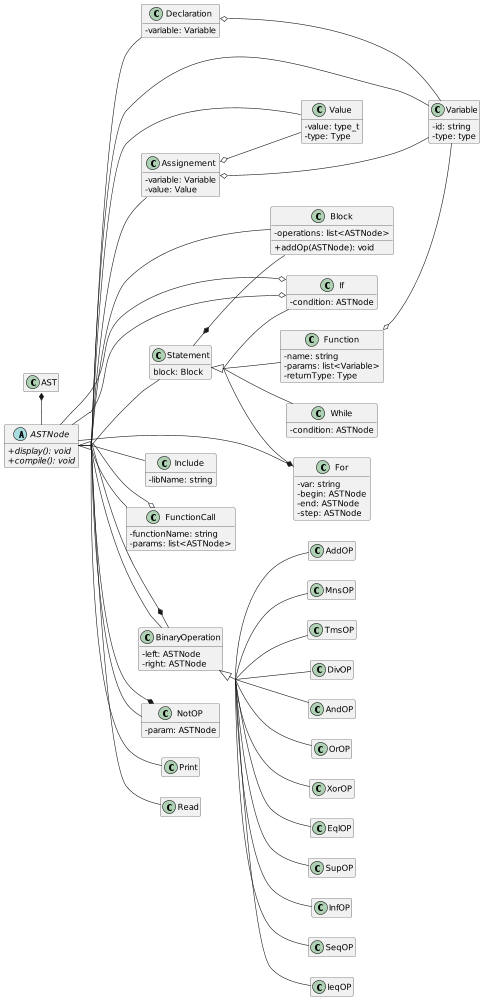
\includegraphics[scale=0.22]{../ressources/diagrams/ast.png}}
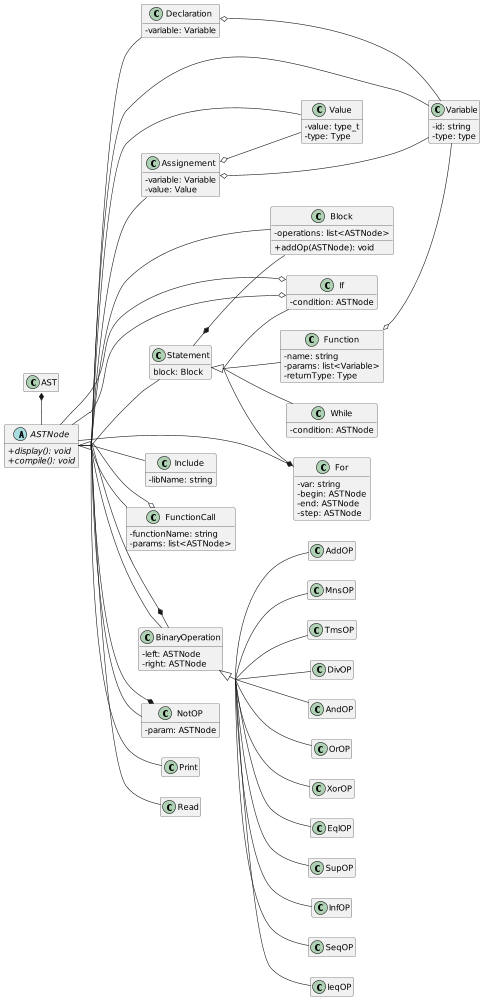
\includegraphics[scale=0.65]{../ressources/diagrams/ast.png}
\end{center}

\clearpage{}
\section{Diagramme de Gantt prévisionnel}\label{appendix:expectedgantt}

\begin{figure}[h!]
  \begin{center}
  \rotatebox[origin=c]{90}{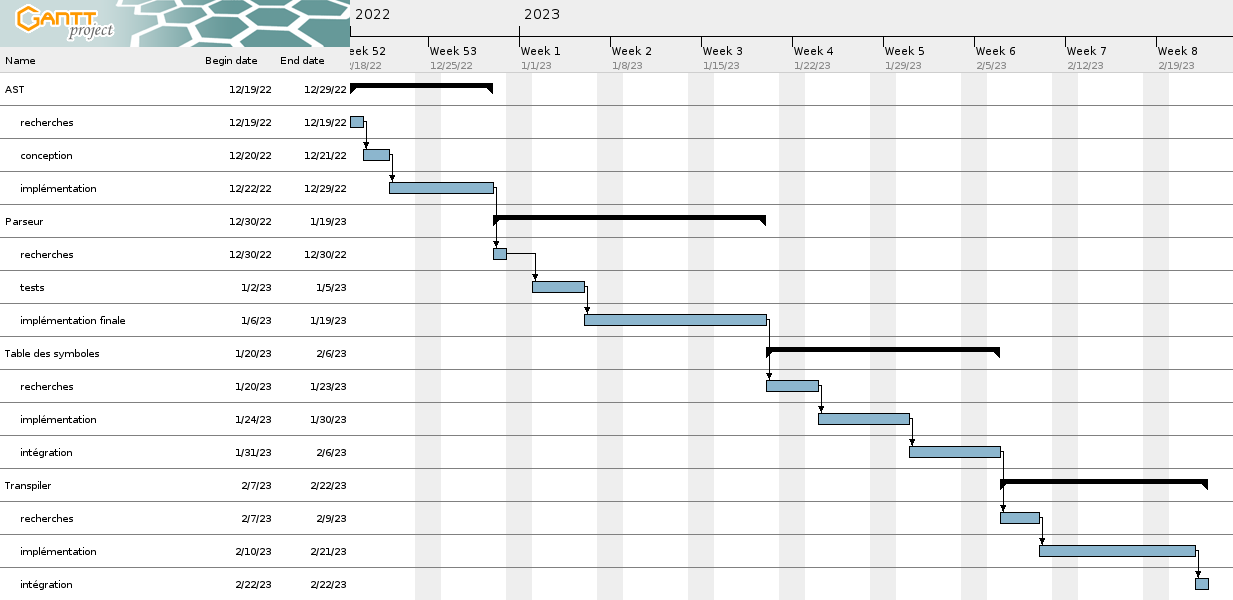
\includegraphics[scale=0.5]{./img/expected-gantt.png}}
  \caption{Diagramme de Gantt prévisionnel.}
  \end{center}
\end{figure}

\clearpage{}
\section{Diagramme de Gantt réel}\label{appendix:realgantt}

\begin{figure}[h!]
  \begin{center}
  \rotatebox[origin=c]{90}{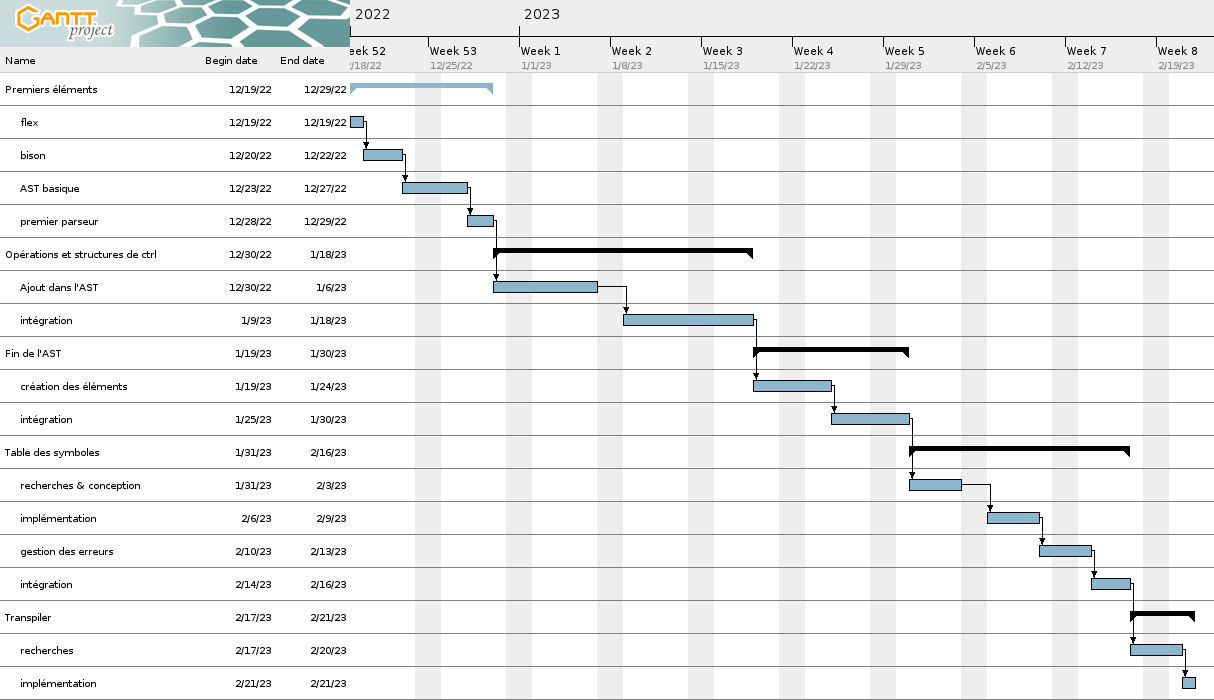
\includegraphics[scale=0.5]{./img/real-project.png}}
  \caption{Diagramme de Gantt réel.}
  \end{center}
\end{figure}

\end{document}


%------------------------------------------------------------------------------%
%               Résumé des réfs (à supprimer à la dernière version
%------------------------------------------------------------------------------%
% \section{Résumé des références}{{{
%
% \begin{itemize}
%   \item La partie consultable de \cite{flexBisonHandbook} présentent les bases
%     de flex.
%   \item \cite{compilerFlexBison} présente la construction d'un compilateur avec
%     flex et bison. Le compilateur présenté utilise une \textbf{table des
%     symboles} ainsi qu'une sorte de \textbf{byte code}. Nous avons choisi
%     l'autre méthode qui consiste à utiliser un object-ABS plutot que directement
%     du byte code. Article très utilisé au départ pour la mise en place du
%     parseur/lexeur.
%   \item \cite{flexmanual}: manuel d'utilisation de Flex.
%   \item \cite{cppparsing}: nous a permis d'avoir un exemple de code qui allie
%     flex et bison en C++ et non en C.
%
%
%   \item \cite{compilerTICH} explication du fonctionnement d'un compilateur.
%   \item \cite{compilerTILB} première version de l'article précédent.
%   \item \cite{crew1997astlog} création d'un analyser syntaxique pour du C/C++:
%     ASTROLOG. L'article par d'analyse syntaxique et de la construction
%     d'\textbf{ABS}.
%
%   \item \cite{visser2002meta} L'objectif de l'article est de présenter
%     l'utilisation des \textbf{ABS} pour de la méta programmation. Il comporte
%     pas mal d'exemples sur les \textbf{ABS} donc je le trouve pertinant.
%   \item \cite{gagnon1998sablecc}: \textbf{ABS} en java.
% \end{itemize}
%
%
% \clearpage{}
% \setcounter{secnumdepth}{1}}}}
